% Pro kompilaci po částech (viz projekt.tex), nutno odkomentovat a upravit
%\documentclass[../projekt.tex]{subfiles}
%\begin{document}

\chapter{Úvod}

\chapter{Vizualizácia dát z~mobilných mapovacích systémov}

Výstupom mobilného mapovacieho systému je množstvo dát z~rôznych senzorov. Dáta, ktoré boli poskytnuté k~tvorbe tejto práce, obsahovali v~prvom rade mračná bodov získané z~lidaru. Aby bolo možné s~týmito mračnami bodov pracovať a vhodne ich zobrazovať, je potrebné, aby mobilný mapovací systém zaznamenával údaje o~svojej polohe. V~tomto prípade boli k~dispozícii údaje o~transláciách a rotáciách kamery s~časovými razítkami. Ďalej býva súčasťou mobilného mapovacieho systému klasická kamera. Pre zobrazenie mračna bodov takým spôsobom, aby sa zobrazenie čo najviac zhodovalo s~kamerovým záznamom, je nutné poznať parametre kamery -- kalibračnú maticu a prípadne aj parametre skreslenia.

Pri vývoji aplikácie, ktorá má umožniť vizualizáciu týchto dát a navyše aj ďalších vektorových dát, je nutné poznať základné princípy zobrazovania 3D dát v~počítačovej grafike. Ďalej je potrebné vybrať si a naštudovať technológie, pomocou ktorých bude aplikácia vytvorená, a to konkrétne niektorý z~frameworkov pre tvorbu aplikácií v~jazyku Python a vhodný framework pre zobrazenie grafických dát. Práve to je predmetom tejto kapitoly.

\section{Dierkový model kamery}

Kamera je v~počítačovej grafike pojem, ktorý označuje projekciu bodov z~trojrozmerného priestoru do roviny. Túto projekciu je možné vyjadriť pomocou matíc a je väčšinou bodová (\emph{central projection}).

Existuje niekoľko rôznych modelov kamery, z~ktorých najjednoduchší je dierkový model kamery (\emph{pinhole camera model}). U~tohto modelu je stred projekcie $\mathbf{C}$  (\emph{camera centre}) v~počiatku Euklidovského súradnicového systému a body sa premietajú do roviny $z = f$, ktorá sa označuje ako obrazová rovina (\emph{image plane}).

Princíp zobrazenia je nasledovný: obrazom bodu $\mathbf{X} = (X, Y, Z)^T$ je bod $\mathbf{x}$, kde priamka vedúca bodom $\mathbf{X}$ a stredom projekcie $\mathbf{C}$ pretína obrazovú rovinu (obrázok \ref{fig:model_kamery1}). Z~podobnosti trojuholníkov je možné odvodiť, že bod $\mathbf{x}$ má súradnice $(fX/Z, fY/Z, f)^T$, postup je naznačený na obrázku \ref{fig:model_kamery2}.

\begin{figure}[h!]
    \centering
    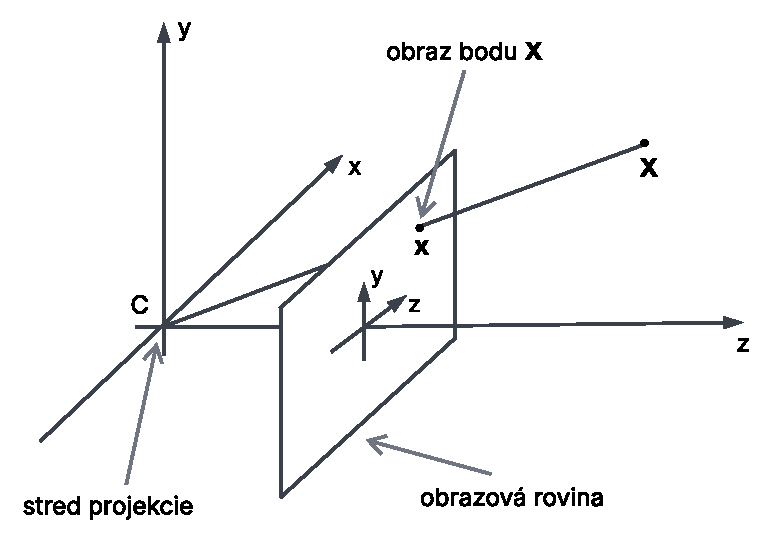
\includegraphics[width=0.7\linewidth]{text_prace/obrazky-figures/model_kamery1.pdf}
    \caption{Zakladný princíp dierkového modelu kamery.}
    \label{fig:model_kamery1}
\end{figure}

\begin{figure}[h!]
    \centering
    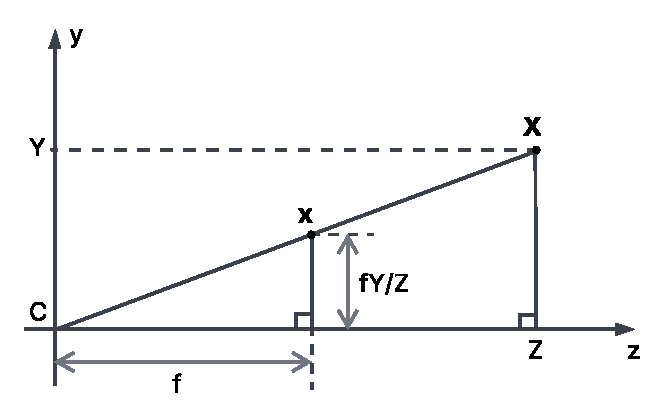
\includegraphics[width=0.7\linewidth]{text_prace/obrazky-figures/model_kamery2.pdf}
    \caption{Náčrt odvodenia súradníc bodu $\mathbf{x}$.}
    \label{fig:model_kamery2}
\end{figure}

Keďže všetky obrazy bodov ležia v~obrazovej rovine $z = f$, je možné poslednú súradnicu zanedbať a zapisovať súradnice bodu $\mathbf{x}$ v~súradnicovom systéme obrazovej roviny ako $(fX/Z, fY/Z)^T$.

Túto projekciu môžeme v~homogénnych súradniciach zapísať pomocou násobenia matíc nasledovným spôsobom:

$$ \mathbf{x} 
=
\begin{pmatrix}
fX \\
fY \\
Z
\end{pmatrix}
=
\begin{bmatrix}
f &   &   & 0 \\
  & f &   & 0 \\
  &   & 1 & 0
\end{bmatrix}
\begin{pmatrix}
X \\
Y \\
Z \\
1
\end{pmatrix}
=
\begin{bmatrix}
f &   &   & 0 \\
  & f &   & 0 \\
  &   & 1 & 0
\end{bmatrix}
\mathbf{X}
=
\mathrm{P} \mathbf{X}
$$

Maticu $\mathrm{P}$ nazývame projekčnou maticou kamery (\emph{camera projection matrix}).

\subsubsection{Rozšírenia základného dierkového modelu kamery}

V~praxi väčšinou chceme vyjadriť body na obrazovej rovine v~súradnicovom systéme, ktorý nemá stred v~bode $(0, 0, f)^T$, ale v~ľubovoľnom bode $(-p_x, -p_y, f)^T$ (obrázok \ref{fig:model_kamery3}). Obrazom bodu $\mathbf{X} = (X, Y, Z)^T$ (v~súradnicovom systéme kamery) potom bude bod $\mathbf{x} = (fX/Z + p_x, fY/Z + p_y, f)^T$ (v~súradnicovom systéme obrazovej roviny). To je možné zahrnúť do projekčnej matice nasledovným spôsobom:

$$ \mathrm{P} =
\begin{bmatrix}
f &   & p_x & 0 \\
  & f & p_y & 0 \\
  &   &  1  & 0
\end{bmatrix}
$$

$$ \mathbf{x} 
=
\begin{pmatrix}
fX/Z + p_x \\
fY/Z + p_y \\
1
\end{pmatrix}
=
\begin{pmatrix}
fX + Z p_x \\
fY + Z p_y \\
Z
\end{pmatrix}
=
\begin{bmatrix}
f &   &  p_x & 0 \\
  & f &  p_y & 0 \\
  &   &   1  & 0
\end{bmatrix}
\begin{pmatrix}
X \\
Y \\
Z \\
1
\end{pmatrix}
$$

Maticu

$$ \mathrm{K} 
=
\begin{bmatrix}
f &   &  p_x \\
  & f &  p_y \\
  &   &   1  
\end{bmatrix}
$$

nazývame kalibračnou maticou kamery (\emph{camera calibration matrix}) a medzi ňou a projekčnou maticou platí vzťah
$\mathrm{P} = \begin{bmatrix} \mathrm{K} | 0 \end{bmatrix}$, kde $0$ predstavuje nulový stĺpcový vektor.

\begin{figure}[h!]
    \centering
    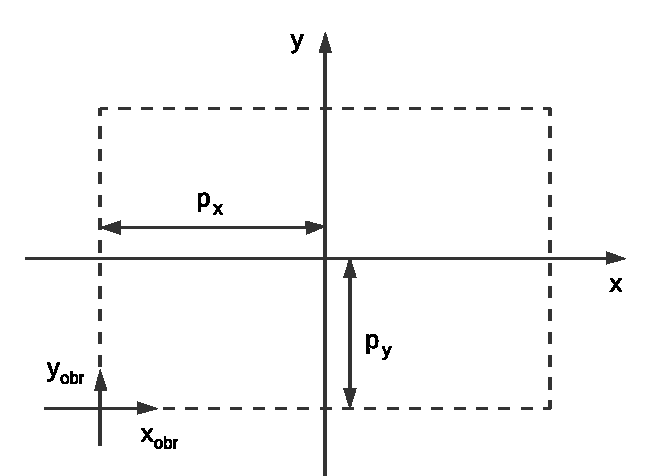
\includegraphics[width=0.7\linewidth]{text_prace/obrazky-figures/model_kamery3.pdf}
    \caption{Súradnicový systém so stredom v~bode $(-p_x, -p_y, f)^T$ obrazovej roviny.}
    \label{fig:model_kamery3}
\end{figure}


Parametre $f$, $p_x$ a $p_y$ označujeme ako \textbf{vnútorné parametre kamery}.

Až doteraz sme predpokladali, že kamera má stred v~počiatku súradnicovej sústavy a je \uv{otočená} v~smere osi $z$, t. j. že obrazová rovina je rovnobežná s~rovinou $xy$. V~praxi to tak však nebýva a kamera má v~súradnicovom systéme, v~ktorom sú definované zobrazované body, istú rotáciu a transláciu. V~takom prípade rozlišujeme všeobecný súradnicový systém a súradnicový systém kamery (\emph{world coordinate frame} a \emph{camera coordinate frame}).

Ak $\widetilde{\mathbf{X}}$ je vektor súradníc bodu $\mathbf{X}$ vo všeobecnom súradnicovom systéme a vektor $\widetilde{\mathbf{X}}_{\mathrm{cam}}$ reprezentuje ten istý bod v~súradnicovom systéme kamery, tak platí vzťah 
$$\widetilde{\mathbf{X}}_{\mathrm{cam}} = \mathrm{R} (\widetilde{\mathbf{X}} - \widetilde{\mathbf{C}}),$$ 
kde $\widetilde{\mathbf{C}}$ sú súradnice stredu kamery vo všeobecnom súradnicovom systéme a $\mathrm{R}$ je rotačná matica $3 \times 3$ reprezentujúca orientáciu súradnicového systému kamery. To vedie k~novému vyjadreniu projekčnej matice ako $\mathrm{P} = \mathrm{K} \mathrm{R} \bigl[ \mathrm{I} | - \widetilde{\mathbf{C}} \bigr]$, kde $\mathrm{I}$ je jednotková matica $3 \times 3$.

Parametre $\mathrm{R}$ a $\widetilde{\mathbf{C}}$ označujeme ako \textbf{vonkajšie parametre kamery}.

Zdrojom všetkých informácií, ktoré boli uvedené v~tejto sekcii, je kniha \emph{Multiple View Geometry in Computer Vision} od autorov R. Hartley a A. Zisserman \cite{multiple_view_geometry}. Odtiaľ sú prevzaté aj obrázky.

\section{Skreslenie kamery}

[parametre skreslenia, výpočet]

\section{Vykresľovací reťazec}

[world space, view space, clip space, screen space, view matrix, projection matrix, viewport transform, vzťah k~dierkovému modelu kamery]


\section{Framework deck.gl a jeho nadstavba Pydeck}
\label{sec:deck_gl}

Pri vývoji webovej aplikácie pre vizualizáciu väčšieho množstva dát, u~ktorej má vykresľovanie prebiehať na strane klienta, teda vo webovom prehliadači, sa hodí priamo či nepriamo použiť niektorý z~frameworkov pre zobrazovanie dát v~jazyku JavaScript.

Takým vhodným frameworkom je napríklad deck.gl, ktorý je určený na zobrazovanie veľkých sád dát. Je zameraný najmä na zobrazovanie geografických dát mapových podkladoch, ale hodí sa aj na iné typy dát. Vyznačuje sa vysokou presnosťou a výkonnosťou. Pre akceleráciu využíva rozhrania WebGPU a WebGL2 \cite{deck.gl_documentation}.

Vizualizácia dát v~deck.gl sa skladá z~dvoch základných častí:
\begin{itemize}
    \item Vrstvy (\texttt{Layers}). Do vrstiev sa ukladajú zobrazované dáta. Framework deck.gl ponúka vyše 30 preddefinovaných typov vrstiev, ktoré zodpovedajú rôznym často sa vyskytujúcim typom dát. Pre túto prácu je významná najmä vrstva \texttt{PointCloudLayer}, ktorá je určená na zobrazenie mračna bodov, a vrstva \texttt{PathLayer}, ktorá je určená na zobrazenie trás.
    \item Pohľad (\texttt{View}). Definuje vlastnosti kamery, napríklad zorné pole a prednú a zadnú orezávaciu rovinu (\emph{near plane} a \emph{far plane}). Je možné buď určiť všetky tieto vlastnosti osobitne, alebo rovno zadať vypočítanú projekčnú maticu.
    Časť \texttt{ViewState} určuje polohu a orientáciu kamery, pričom u~orientácie je možné určiť iba dva uhly (\emph{bearing} a \emph{pitch}). Typ pohľadu definuje spôsob interakcie vizualizácie s~používateľom, napríklad pre zobrazenie trate z~pohľadu strojvedúceho je ideálny typ \texttt{FirstPersonView}.
\end{itemize}

To, že sa deck.gl na vizualizáciu dát z~mobilného mapovacieho systému naozaj hodí, dokazujú ukážky na jeho webových stránkach. Použiteľnosť vrstvy \texttt{PointCloudLayer} demonštruje plynulá animácia mračna vyše 800~000 bodov.

Na webových stránkach deck.gl sa nachádza aj galéria projektov vytvorených pomocou tohto frameworku. Medzi nimi je Autonomous Visualization System, toolkit pre vývoj webových aplikácií pre vizualizáciu dát z~autonómnych vozidiel \cite{avs}. Na webových stránkach tohto projektu je ukážka takej aplikácie, ktorá zobrazuje vozidlo, dáta z~lidaru, vektorové dáta, ako napríklad trasu vozidla, a záznam z~kamery. To je veľmi podobné aplikácii vyvíjanej v~rámci tejto práce, ale je tu niekoľko rozdielov. Poprvé, mračno bodov nie je agregované, a teda sa v~každom kroku animácie zobrazuje iba v~tom momente nasnímaná časť, a podruhé, kamerový záznam sa zobrazuje oddelene, a nie na pozadí mračna bodov a vektorových dát.

Hoci je framework deck.gl primárne určený pre použitie v~Javascripte, je možné ho použiť aj v~jazyku Python, a to pomocou knižnice \textbf{Pydeck}. Tá je pomerne jednoduchá a podstatou jej činnosti je, že prevedie kód napísaný v~jazyku Python do formátu JSON. Framework deck.gl má totiž modul @deck.gl/json, ktorý prijíma reprezentáciu vizualizácie vo formáte JSON a transformuje ju do javascriptového kódu (na definície funkcií a deck.gl objektov)\footnote{Ukážka rozhrania modulu @deck.gl/json je na \url{https://deck.gl/playground}.}.

Knižnica Pydeck je dobrým prostriedkom na vytvorenie jednoduchých vizualizácií, s~ktorými môže používateľ interagovať pohybmi myši. Jej možnosti sú však oproti pôvodnému frameworku deck.gl veľmi obmedzené. Nie je vhodná na vytváranie zložitejších animácií s~veľkým množstvom dát, pretože sa aj po tej najmenšej zmene musia dáta a definícia vizualizácie nanovo prevádzať do formátu JSON a následne na javascriptový kód (obrázok \ref{fig:pydeck_dashdeck_schema}), čo je veľmi časovo náročné.

\begin{figure}[h]
    \centering
    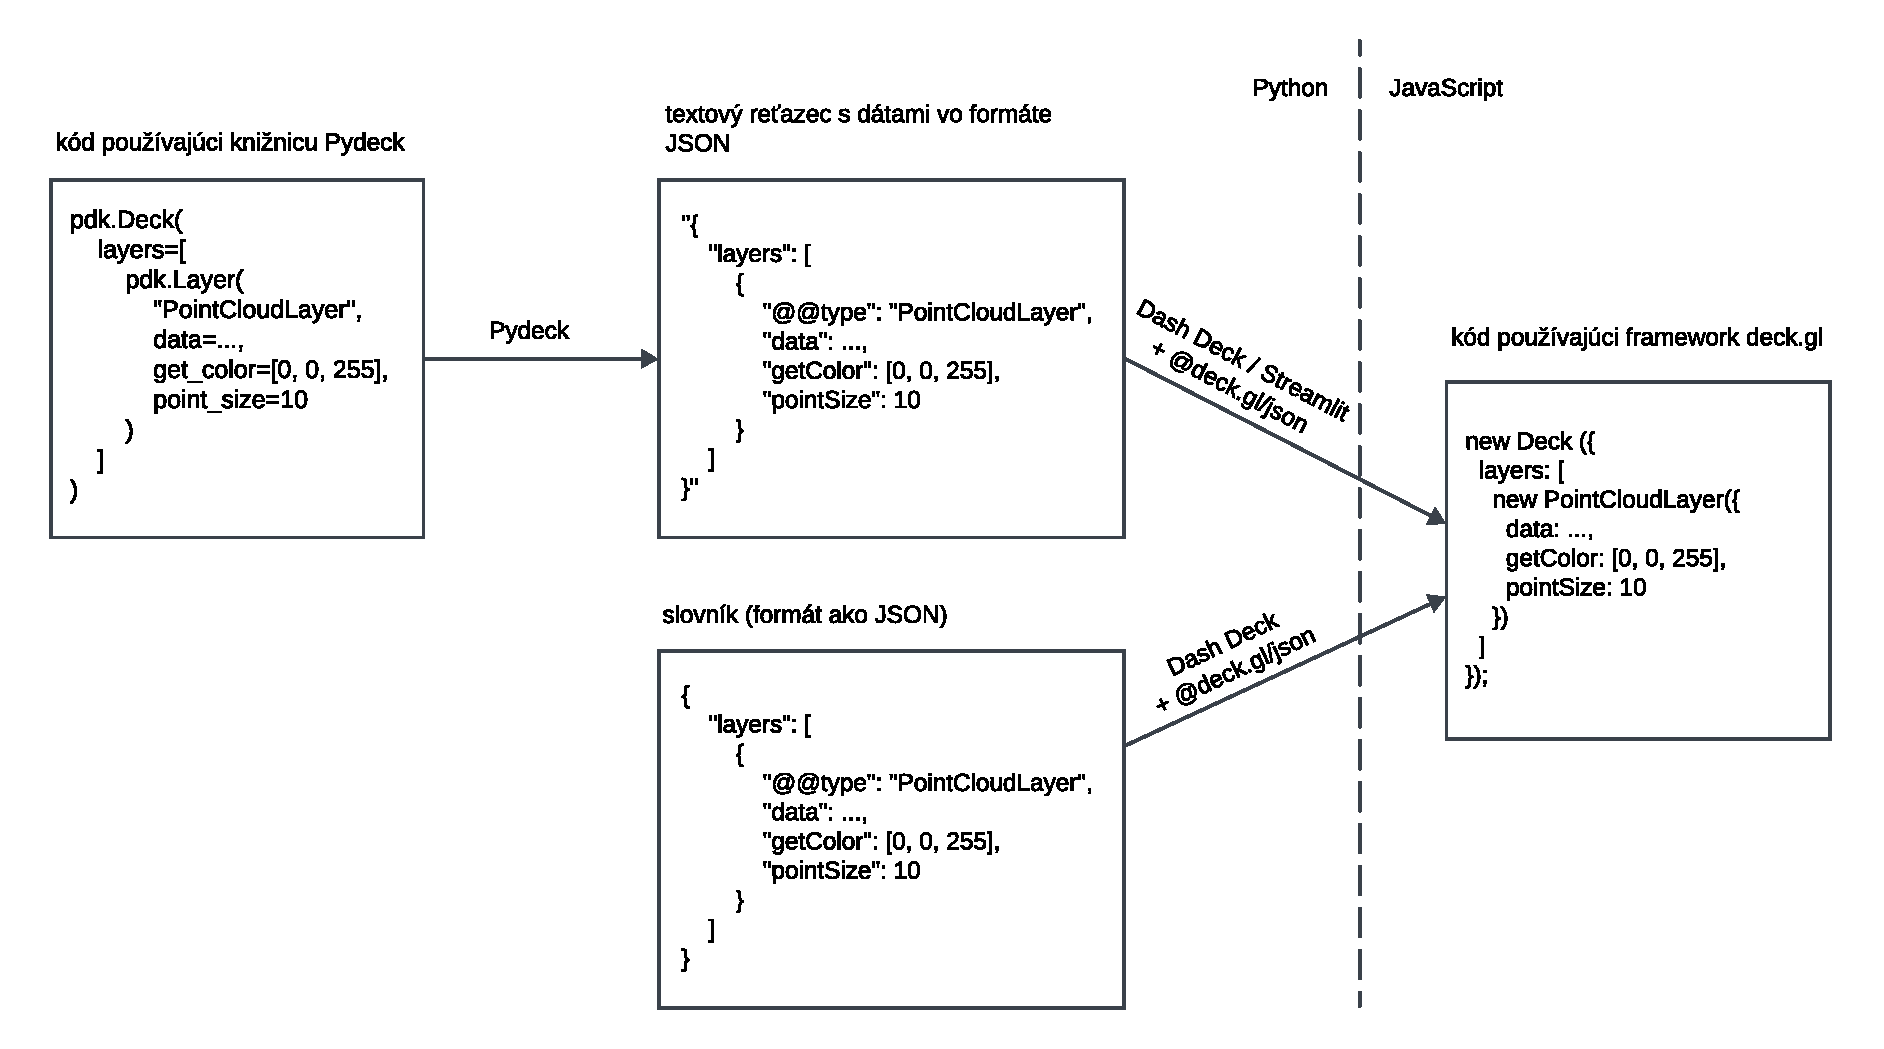
\includegraphics[width=1\linewidth]{text_prace/obrazky-figures/pydeck_dashdeck_transformacie.pdf}
    \caption{Schéma vzťahov medzi technológiami Pydeck, Dash Deck a deck.gl a transformácií, ktorými prechádza definícia zobrazenia.}
    \label{fig:pydeck_dashdeck_schema}
\end{figure}

\section{Nastavenie polohy kamery vo frameworku deck.gl}
\label{sec:nastavenie_polohy_kamery}

Súčasťou dodaných dát z~mobilného mapovacieho systému boli rotácie a translácie kamery. Pre nastavenie polohy vo frameworku deck.gl existujú dve možnosti:

\begin{enumerate}
    \item Aplikovať transformáciu na dáta a nechať kameru v~počiatku súradnicového systému, prípadne v~nejakom inom pevnom bode.
    \item Nechať dáta v~pôvodnom stave a aplikovať všetky transformácie iba na kameru.
\end{enumerate}

Je zrejmé, že pre dosiahnutie rovnakého výsledku musí byť transformácia použitá v~druhom prípade inverzná k~tej, ktorá je použitá v~tom prvom.

Bližším popisom a zhodnotením výhod a nevýhod týchto dvoch metód sa zaoberajú nasledujúce dve podsekcie.

\subsubsection{Aplikovanie transformácií na dáta}

Ako bolo zmienené v~sekcii \ref{sec:deck_gl}, dáta sa vo frameworku deck.gl členia do vrstiev. Každej vrstve je potom potrebné priradiť pole s~dátami a definovať pre ňu takzvané prístupové funkcie (\emph{data accessors}), ktoré určujú, akým spôsobom sa z~poľa s~dátami získa poloha a farba prvku. Napríklad u~vrstvy \texttt{PointCloudLayer} je potrebné definovať funkciu \texttt{getPosition} pre získanie polohy bodu a \texttt{getColor} pre výpočet farby bodu \cite{deck.gl_documentation}.

Práve vo funkcii \texttt{getPosition} je možné aplikovať na polohu bodu ľubovoľnú transformáciu.

Napríklad v~prípade, že je potrebné posunúť kameru v~mračne bodov o~10 jednotiek v~kladnom smere po osi x, by bolo možné vykonať túto transformáciu pomocou funkcie \texttt{getPosition} tak, že by sa posunul každý bod po osi x o~10 jednotiek v~zápornom smere. V~prípade, že by bol v~poli dát každý bod vo formáte \texttt{[x, y, z, intenzita]}, by potom funkcia \texttt{getPosition} vyzerala takto:

\begin{lstlisting}
function getPosition(d) {
  return [d[0] - 10, d[1], d[2]];
}
\end{lstlisting}

Výhodou tohto prístupu je, že je možné vykonať ľubovoľnú transformáciu, pretože do funkcie možno napísať akýkoľvek kód.

Veľkou nevýhodou je časová náročnosť, pri zmene polohy kamery sa totiž musí prepočítať poloha každého bodu. Tieto výpočty sa vykonávajú na procesore a výsledky sa následne nahrávajú na grafickú kartu. To konštatuje aj samotná dokumentácia frameworku deck.gl, kde sa píše, že kľúčom k~tvorbe výkonných aplikácií je minimalizácia aktualizácií vrstiev, pri ktorých dochádza k~prepočítavaniu dát a ich opätovnému nahrávaniu na grafickú kartu. Taktiež je tam uvedené, že prístupové funkcie by mali byť čo najtriviálnejšie, pretože sa počítajú pre každú položku v~dátach, t. j. pre každý bod v~mračne bodov, a teda sa každé pridanie operácií naviac výrazne prejaví na výkonnosti. 99\% procesorového času venovaného aktualizácii dát vrstvy sa strávi práve volaním prístupových funkcií \cite{deck.gl_performance_optimization}.

\subsubsection{Aplikovanie transformácií na kameru}

Meniť polohu a orientáciu kamery je v~deck.gl možné pomocou troch parametrov: \texttt{position}, \texttt{bearing} a \texttt{pitch} \cite{deck.gl_documentation}. To sú rotácie iba podľa dvoch osí, a teda nie je možné dosiahnuť všeobecnú rotáciu -- chýba možnosť nastaviť rotáciu okolo tretej osi, takzvaný \emph{roll} uhol.

V~dokumentácii deck.gl je popísaná aj trieda \texttt{Viewport}, u~ktorej je možné namiesto parametrov \texttt{position}, \texttt{bearing} a \texttt{pitch} nastaviť maticu pohľadu \texttt{viewMatrix}, čo znamená možnosť použiť akúkoľvek rotáciu. Problém je však v~tom, že sa v~dokumentácii už nikde nepíše, ako túto triedu použiť. Ide teda o~nezrovnalosť, pravdepodobne pozostatok z~predchádzajúcich verzií deck.gl, kde táto možnosť bola, ale medzičasom bola zrušená. V~aktuálnej verzii je možné túto maticu už iba prečítať, ale nie nahradiť vlastnou.

Nevýhodou tohto spôsobu nastavenia polohy kamery teda je, že sa nedá nastaviť \emph{roll} uhol. Tento problém je však možné vyriešiť trikom, a to otočením HTML elementu \texttt{canvas}, do ktorého deck.gl vykresľuje výsledné zobrazenie, pomocou CSS vlastnosti \texttt{transform}. 

Za poznámku tiež stojí, že ak potrebujeme na kameru aplikovať nejakú zložitejšiu transformáciu než iba jednu rotáciu a posunutie, tak je potrebné odvodiť vzorce, ktorými sa táto zložitejšia transformácia prevedie na parametre \texttt{position}, \texttt{bearing} a \texttt{pitch}. Konrétnym prípadom, ktorý bolo potrebné vyriešiť v tejto práci, sa zaoberá nasledujúca kapitola.

Veľkou výhodou naopak je, že na rozdiel od predchádzajúceho spôsobu nedochádza k~žianym aktualizáciám vrstiev, teda nie je potrebné prepočítavať polohy bodov na procesore ani ich znova nahrávať na grafickú kartu. Tým sa výrazne zvýši výkonnosť.

\subsubsection{Upresnenie polohy kamery}

Experimentmi s dodanými dátami sa zistilo, že ak je mračno bodov zobrazené presne podľa dodaných údajov o polohe a parametroch kamery, výsledné zobrazenie nesedí presne na záber z kamery. Aby naozaj sedelo, je potrebné pridať isté posunutie kamery. Taká situácia je zjednodušene znázornená na obrázku \ref{fig:transformacie_kamery} -- je zadaná translácia $T$ a rotácia $R$, ale kameru je ešte potrebné posunúť doprava transláciou $T'$.

\begin{figure}[h]
    \centering
    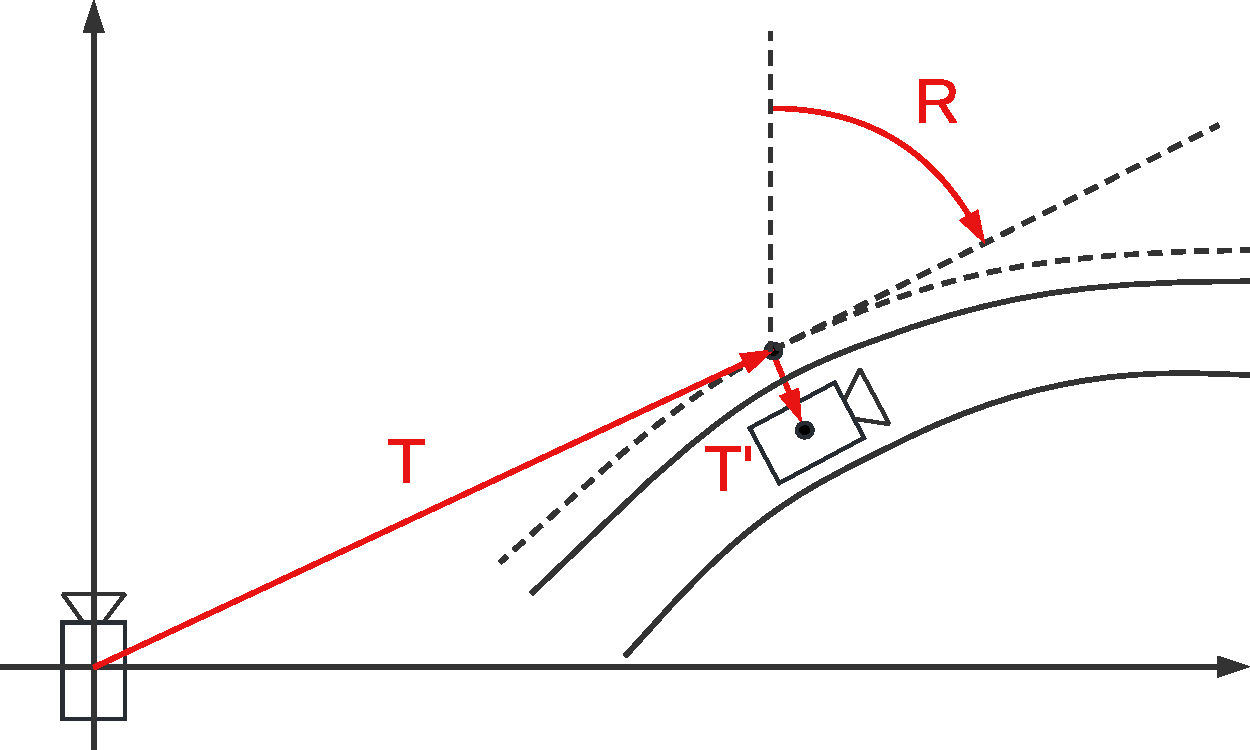
\includegraphics[width=0.8\linewidth]{text_prace/obrazky-figures/tri_transformacie.pdf}
    \caption{Zjednodušený príklad situácie, kedy je potrebné kombinovať viacero transformácií kamery. Je k~dispozícii translácia $T$ a rotácia $R$, ale kameru je ešte potrebné posunúť doprava transláciou $T'$, aby bola v~strede koľajníc.}
    \label{fig:transformacie_kamery}
\end{figure}

Ak by bolo pri implementácii v deck.gl možné použiť aplikovanie transformácií na dáta, mal by tento problém jednoduché riešenie: z~translácie $T$ a rotácie $R$ sa zloží transformačná matica, ktorá sa použije v~prístupovej funkcii, a translácia $T'$ sa priamo použije ako poloha kamery.

Ak však tento prístup nie je vhodný, napríklad z dôvodu horšieho výkonu, je nutné nájsť transláciu $T_V$ a rotáciu $R_V$ tak, aby platil vzťah 

$$ T R T' = T_V R_V \mathrm{.}$$

Transformácie $T_V$ a $R_V$ sa potom už totiž dajú priamo previesť na parametre \texttt{position}, \texttt{bearing} a \texttt{pitch} (na prevod rotácie na \texttt{bearing} a \texttt{pitch} sa dá použiť napríklad trieda \texttt{Rotation} z knižnice \texttt{scipy}).

Nech

$$
    T =
    \begin{pmatrix}
    1 & 0 & 0 & t_1 \\
    0 & 1 & 0 & t_2 \\
    0 & 0 & 1 & t_3 \\
    0 & 0 & 0 & 1
    \end{pmatrix}
    \mathrm{,} \quad 
    R =
    \begin{pmatrix}
    r_{11} & r_{12} & r_{13} & 0 \\
    r_{21} & r_{22} & r_{23} & 0 \\
    r_{31} & r_{32} & r_{33} & 0 \\
    0 & 0 & 0 & 1
    \end{pmatrix}
    \mathrm{,} \quad 
    T' =
    \begin{pmatrix}
    1 & 0 & 0 & t'_1 \\
    0 & 1 & 0 & t'_2 \\
    0 & 0 & 1 & t'_3 \\
    0 & 0 & 0 & 1
    \end{pmatrix}
    \mathrm{,}
$$
$$
    T_V =
    \begin{pmatrix}
    1 & 0 & 0 & t_{v1} \\
    0 & 1 & 0 & t_{v2} \\
    0 & 0 & 1 & t_{v3} \\
    0 & 0 & 0 & 1
    \end{pmatrix}
    \quad \mathrm{a} \quad 
    R_V =
    \begin{pmatrix}
    r_{v11} & r_{v12} & r_{v13} & 0 \\
    r_{v21} & r_{v22} & r_{v23} & 0 \\
    r_{v31} & r_{v32} & r_{v33} & 0 \\
    0 & 0 & 0 & 1
    \end{pmatrix}
    \mathrm{.}
$$

Potom

$$
    T R T' =
    \begin{pmatrix}
    r_{11} & r_{12} & r_{13} & t'_1 r_{11} + t'_2 r_{12} + t'_3 r_{13} + t_1 \\
    r_{21} & r_{22} & r_{23} &  t'_1 r_{21} + t'_2 r_{22} + t'_3 r_{23} + t_2 \\
    r_{31} & r_{32} & r_{33} &  t'_1 r_{31} + t'_2 r_{32} + t'_3 r_{33} + t_3 \\
    0 & 0 & 0 & 1
    \end{pmatrix}
$$

a

$$
    T_V R_V =
    \begin{pmatrix}
    r_{v11} & r_{v12} & r_{v13} & t_{v1} \\
    r_{v21} & r_{v22} & r_{v23} & t_{v2} \\
    r_{v31} & r_{v32} & r_{v33} & t_{v3} \\
    0 & 0 & 0 & 1
    \end{pmatrix} \mathrm{.}
$$

Z toho je vyplýva, že musí platiť $R_V = R$ a

$$
    \begin{pmatrix}
    t_{v1} \\
    t_{v2} \\
    t_{v3} \\
    \end{pmatrix}
    =
    \begin{pmatrix}
    t'_1 r_{11} + t'_2 r_{12} + t'_3 r_{13} + t_1 \\
    t'_1 r_{21} + t'_2 r_{22} + t'_3 r_{23} + t_2 \\
    t'_1 r_{31} + t'_2 r_{32} + t'_3 r_{33} + t_3
    \end{pmatrix}
    =
    \begin{pmatrix}
    r_{v11} & r_{v12} & r_{v13} \\
    r_{v21} & r_{v22} & r_{v23} \\
    r_{v31} & r_{v32} & r_{v33}
    \end{pmatrix}
    \begin{pmatrix}
    t'_1 \\
    t'_2 \\
    t'_3
    \end{pmatrix}
    +
    \begin{pmatrix}
    t_1 \\
    t_2 \\
    t_3
    \end{pmatrix} \mathrm{.}
$$

Tým sme našli hľadanú transláciu $T_V$ a rotáciu $R_V$.

\section{Frameworky pre tvorbu webových aplikácií}

Keďže hlavným cieľom práce bolo vytvoriť aplikáciu v jazyku Python, a to ideálne webovú, bolo potrebné preskúmať existujúce technológie, ktoré to umožňujú.

\subsubsection{Porovnanie frameworkov Streamlit a Dash}

Streamlit a Dash sú frameworky, ktoré majú rovnaké zameranie: oba slúžia na tvorbu webových aplikácií pre prácu s~dátami (\emph{data apps}) v~jazyku Python. Dash je oproti Streamlitu na nižšej úrovni abstrakcie, pretože sám o~sebe nemá žiaden vizuálny štýl a mnohé jeho komponenty sa priamo mapujú na HTML elementy, napríklad \texttt{dash.html.Div} a \texttt{dash.html.H1} \cite{dash_documentation, streamlit_documentation}.

Oba frameworky majú podporu pre Pydeck, u~Streamlitu je priamo k~dispozícii element \texttt{st.pydeck\_chart} a Dash má na tento účel vytvorenú prídavnú knižnicu \textbf{Dash Deck}. Ukázalo sa však, že \texttt{st.pydeck\_chart} podporuje iba pohľad \texttt{MapView}, ktorý je určený na zobrazenie dát na mape a nedá sa použiť na perspektívne zobrazenie bodov v~trojrozmernom priestore. Preto je pre účely tejto práce element \texttt{st.pydeck\_chart} prakticky nepoužiteľný.

Dash Deck má navyše tú výhodu, že umožňuje vynechať Pydeck a definovať zobrazenie iba pomocou slovníkov so štruktúrou zodpovedajúcou tej, ktorú vyžaduje modul @deck.gl/json, čo je tiež znázornené na obrázku \ref{fig:pydeck_dashdeck_schema}. To trochu zefektívni vykonávanie zmien vo vizualizácii, keďže taká reprezentácia umožní jednoduchšie vykonávanie úprav.

Z týchto dôvodov bol pre implementáciu zvolený framework Dash, ktorý je podrobnejšie popísaný v nasledujúcej podsekcii.

\subsubsection{Popis frameworku Dash}

Dash je framework, ktorý umožňuje tvorbu webových aplikácií v~jazyku Python. Vytvorený kód aplikácie sa spúšťa v rámci HTTP servera a generuje HTML dokument a skripty v jazyku JavaScript, ktoré server odošle klientovi. Tieto skripty následne komunikujú sa serverom, čím sa zabezpečuje funkcionalita aplikácie. Server je bezstavový a neuchováva si žiadne informácie o klientoch.

Kód webovej aplikácie napísanej s využitím frameworku Dash sa skladá z dvoch základných častí: komponentov a callbackov.

\emph{Komponenty} sú prvky používateľského rozhrania, ktoré sa skladajú do stromovej štruktúry. Je možné použiť komponenty priamo zodpovedajúce HTML elementom (Dash HTML Components), komponenty z knižnice Dash Core Components (napríklad \texttt{Graph}, \texttt{Input}, \texttt{Tabs}, \texttt{Upload}) a ďalšie špeciálne komponenty \cite{dash_documentation}.

Pre túto prácu je významný komponent \texttt{Store} z knižnice Dash Core Components, ktorý umožňuje uložiť dáta na strane klienta. Hodí sa na uloženie dát, ktoré sa následne zobrazujú pomocou frameworku deck.gl.

Ďalej je možné použiť knižnicu \textbf{Dash Bootstrap Components} (DBC), ktorá poskytuje ďalšie komponenty, ikony, lepšie možnosti pre rozloženie stránky, a v neposlednom rade vizuálne štýly \cite{dbc_documentation}.

Tam, kde nestačia štýly a možnosti rozloženia stránky z DBC, je možné u komponentov dodefinovať vlastné pravidlá v jazyku CSS.

\emph{Callbacky} vytvárajú funkcionalitu aplikácie. Každý callback je funkcia, ktorá má vstupy a výstupy. Vstupy a výstupy sú vždy atribúty konkrétnych komponentov. Callback sa zavolá na začiatku behu aplikácie (táto vlastnosť sa dá zrušiť) a potom vždy, keď sa zmení niektorý z jeho vstupov. Callback môže mať aj špeciálne vstupy typu \texttt{State}, ktorých zmena callback nespustí. Platí obmedzenie, že každý atribút komponentu môže byť výstupom maximálne jedného callbacku \cite{dash_documentation}. U vstupov žiadne obmedzenia nie sú.

Existujú dva typy callbackov.
\begin{itemize}
    \item Obyčajné callbacky. Sú napísané v jazyku Python. Klient má iba informáciu o ich vstupoch a výstupoch. Keď sa zmení niektorý zo vstupov, klient pošle na server požiadavok obsahujúci hodnoty všetkých vstupov. Server spustí kód callbacku a pošle klientovi odpoveď, ktorá obsahuje hodnoty všetkých výstupov.
    \item Klientske callbacky. Sú napísané v jazyku JavaScript. Klient má k dispozícii celý kód callbacku. Keď sa zmení niektorý zo vstupov, klient vykoná kód callbacku bez akejkoľvek komunikácie so serverom.
\end{itemize}

Je zrejmé, že klientske callbacky sú efektívnejšie než tie obyčajné, pretože ich nespomaľuje réžia komunikácie so serverom. Najvýraznejšie sa to prejaví vtedy, keď vstupy alebo výstupy obsahujú veľké množstvo dát.

K aplikácii vytvorenej pomocou frameworku Dash je možné pridať vlastné štýlové predpisy a skripty alebo moduly v jazyku JavaScript. Je potrebné uložiť ich do priečinka s názvom \texttt{assets} v koreňovom priečinku aplikácie. Rovnako je nutné postupovať aj pri vkladaní obrázkov a videí. Všetky štýlové predpisy, skripty a moduly z priečinka \texttt{assets} Dash automaticky načítava a pripája k aplikácii \cite{dash_documentation}.

\chapter{Návrh aplikácie}

Cieľom tejto práce bolo vytvoriť používateľskú aplikáciu. Výsledná aplikácia mala byť webová, aby ju bolo možné spustiť jednoducho pomocou webového prehliadača. Čo sa týka funkcionality, mala by spĺňať nasledujúce body:

\begin{itemize}
    \item Zobrazenie dát z~mobilného mapovacieho systému. Tieto dáta sú tvorené mračnom bodov z~lidaru, kamerovým záznamom, údajmi o~pohybe vlaku a ďalšími vektorovými dátami a mali by byť zobrazené z~pohľadu strojvedúceho vlaku.
    \item Umožniť používateľovi vybrať si konkrétnu pozíciu vlaku alebo prehrať si animáciu pohybu vlaku s nastaviteľnou rýchlosťou.
    \item Umožniť používateľovi nahrať súbory s~dátami na zobrazenie: súbor s~mračnom bodov, video z~kamery na čele vlaku, súbor s~vektorovými dátami, textové súbory s~údajmi o~pohybe vlaku -- pole translácií, pole rotácií a pole zodpovedajúcich časových razítok.
    \item Zobrazovať dva typy dát z~lidaru -- buď malé, postupne nasnímané kusy mračna bodov s~časovými razítkami, alebo iba jedno celistvé mračno bodov, ktoré vzniklo ich spojením (u~oboch typov ale ide o~agregované dáta -- všetky body sú v~jednej spoločnej súradnicovej sústave). Umožniť používateľovi prepínať medzi týmito dvoma typmi.
    \item Poskytnúť používateľovi možnosti prispôsobenia zobrazenia, ako napríklad zmeny viditeľnosti jednotlivých vrstiev (mračno bodov, vektorové dáta, kamerový záznam) a základné nastavenia zobrazenia mračna bodov (rôzne farebné škály podľa intenzity, veľkosť a priehľadnosť bodov, zobrazenie bodov len do určitej vzdialenosti) aj vektorových dát (farba a hrúbka čiar).
    \item Mať prepínač na zapnutie a vypnutie skreslenia mračna bodov a vektorových dát podľa parametrov skreslenia kamery.
    \item Zobrazovať prejazdný profil vlaku v~predikovanej polohe v~rôznych vzdialenostiach pred vlakom -- 25, 50, 75 a 100m. Zobrazovať aj čiaru spájajúcu predikované polohy. (Súbory s predikovanými polohami sú súčasťou dát, ktoré aplikácia načítava.)

\end{itemize}

\section{Návrh používateľského rozhrania}

Pri návrhu používateľského rozhrania aplikácie bolo prioritou zobrazenie vizualizácie ako hlavnej časti aplikácie na čo najväčšej ploche a tiež tak, aby bola viditeľná vo všetkých stavoch.

Z ovládacích prvkov sú za najdôležitejšie považované prvky pre zmenu polohy vlaku, ktoré sú umiestnené v spodnom paneli. Všetky ostatné ovládacie prvky sú skryté v bočnom paneli, ktorý sa dá vysunúť tlačítkom v ľavom hornom rohu, a sú rozdelené do troch záložiek -- nahrávanie dát, prispôsobenie zobrazenia a samostatná záložka pre prejazdný profil. Celkový návrh vzhľadu je na obrázku \ref{fig:navrh_gui}.

\begin{figure}[h]
    \centering
    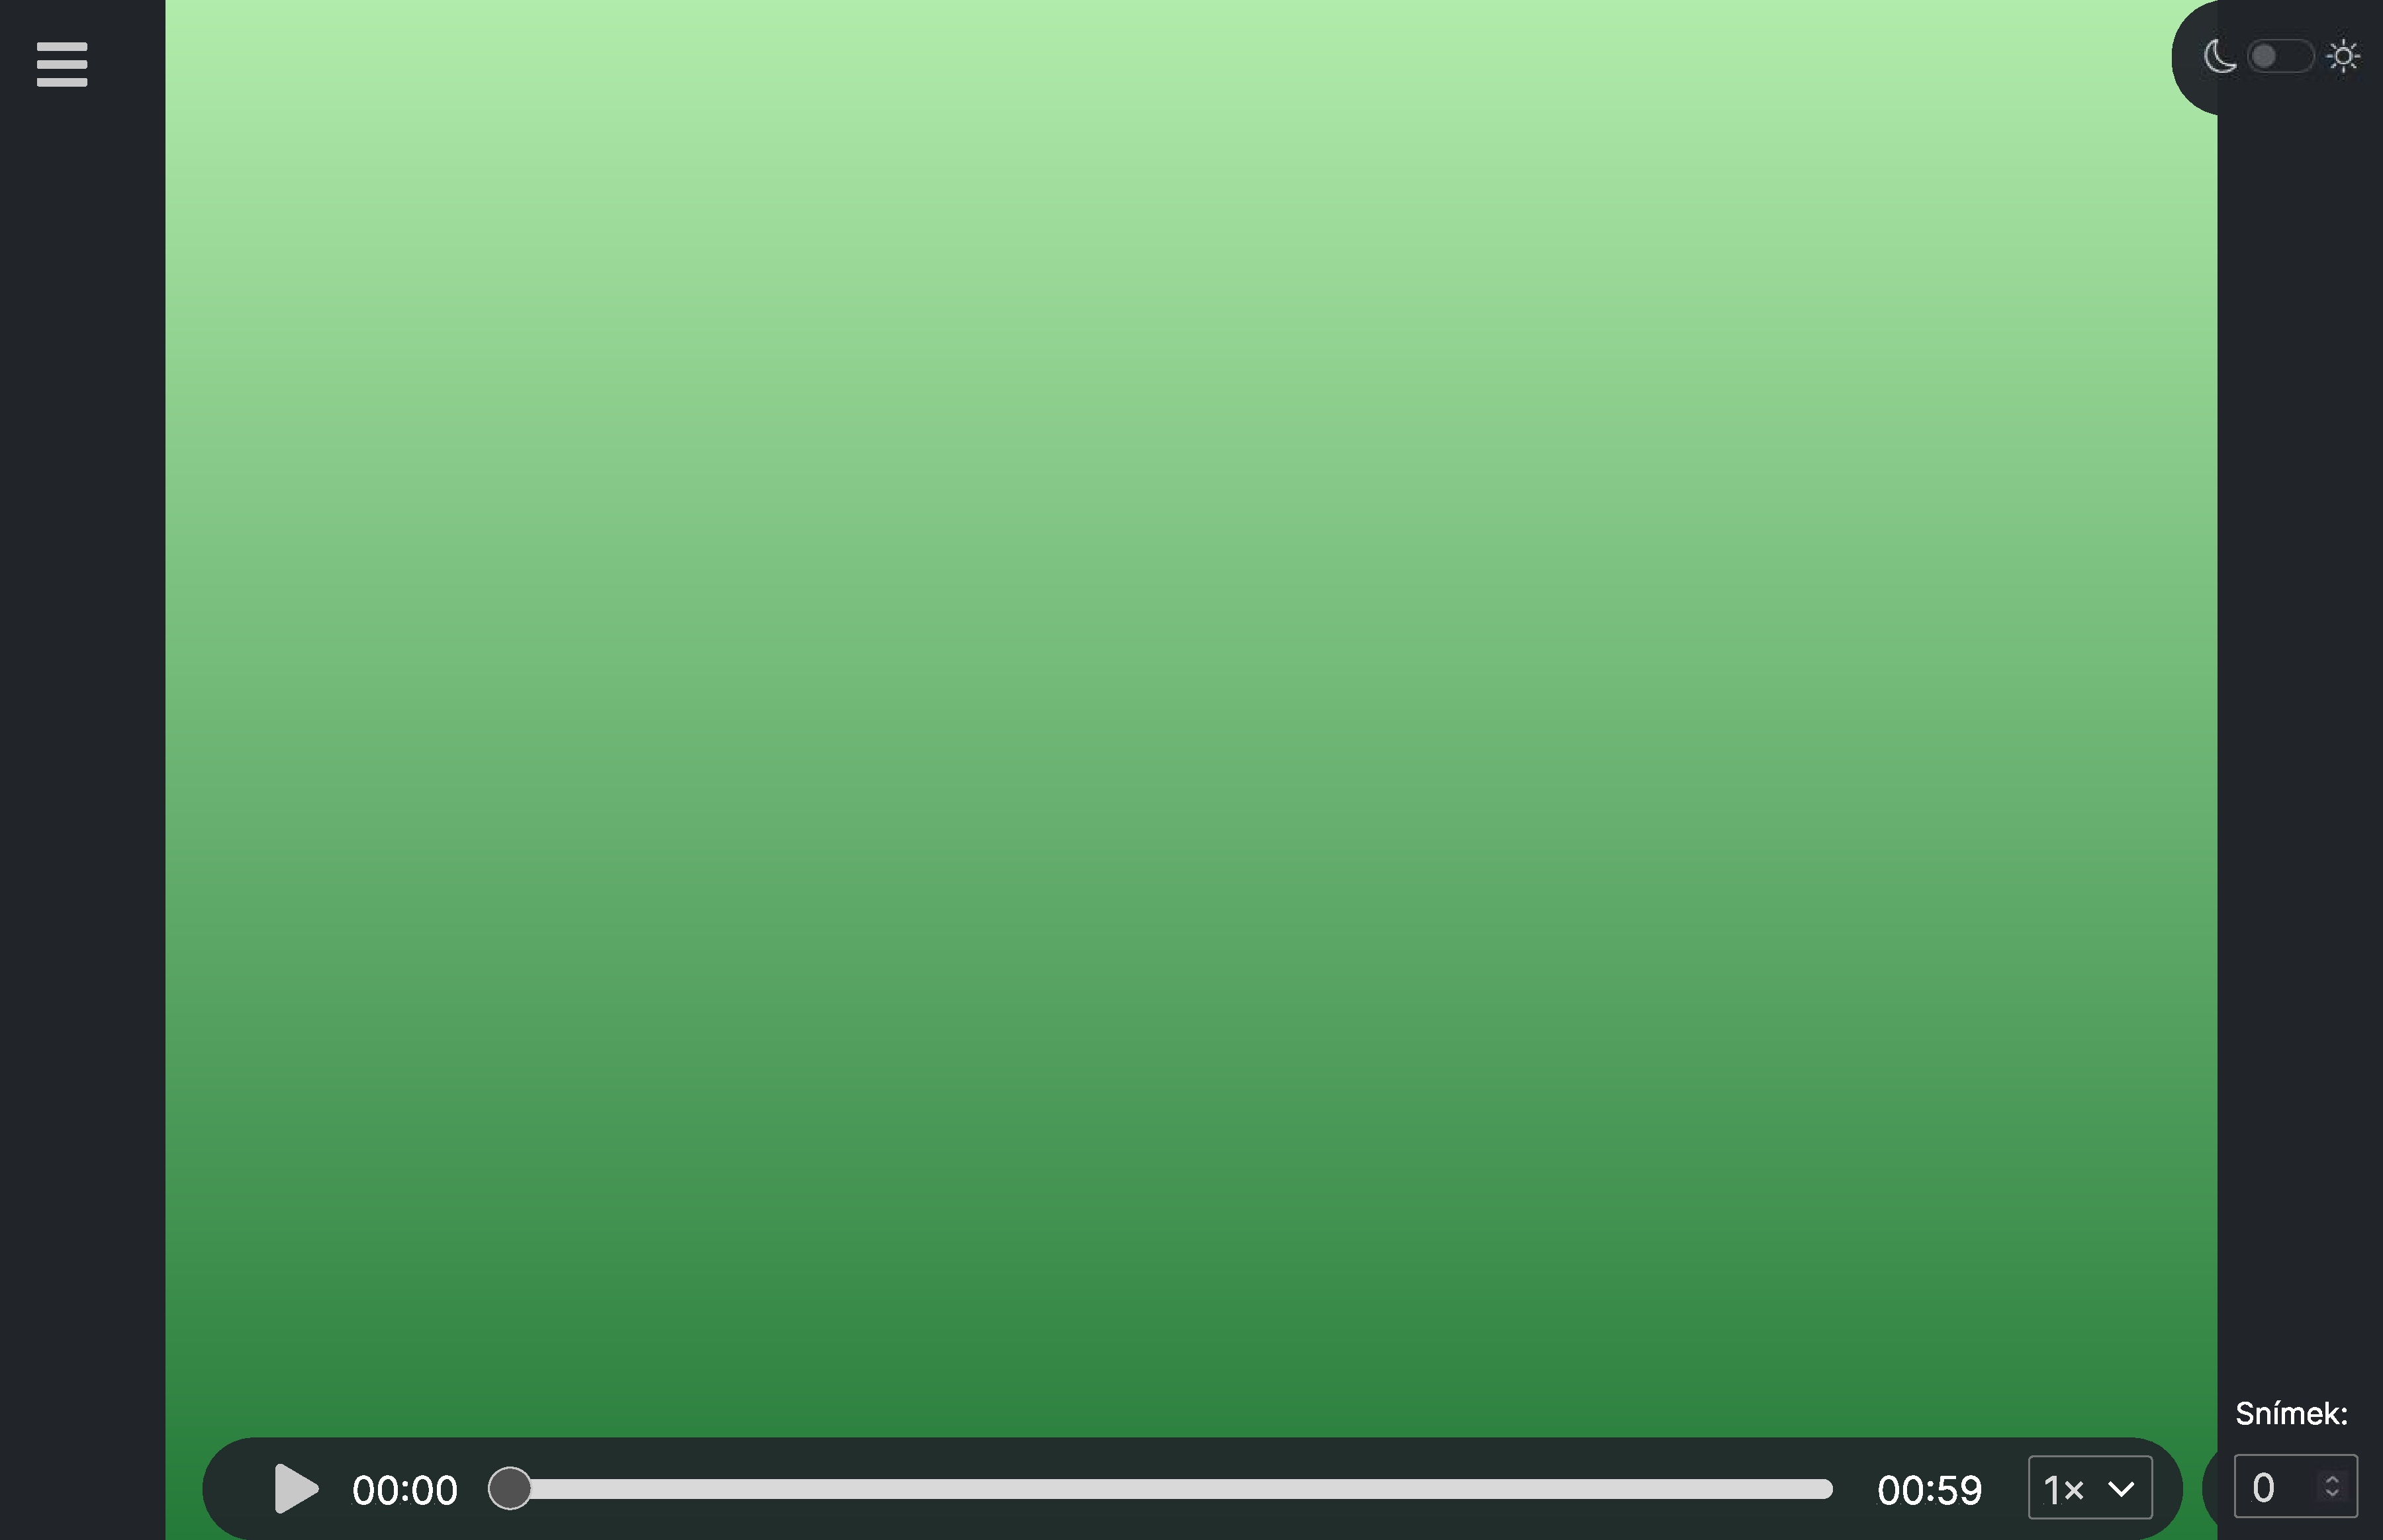
\includegraphics[width=0.9\linewidth]{text_prace/obrazky-figures/navrh1.pdf}
    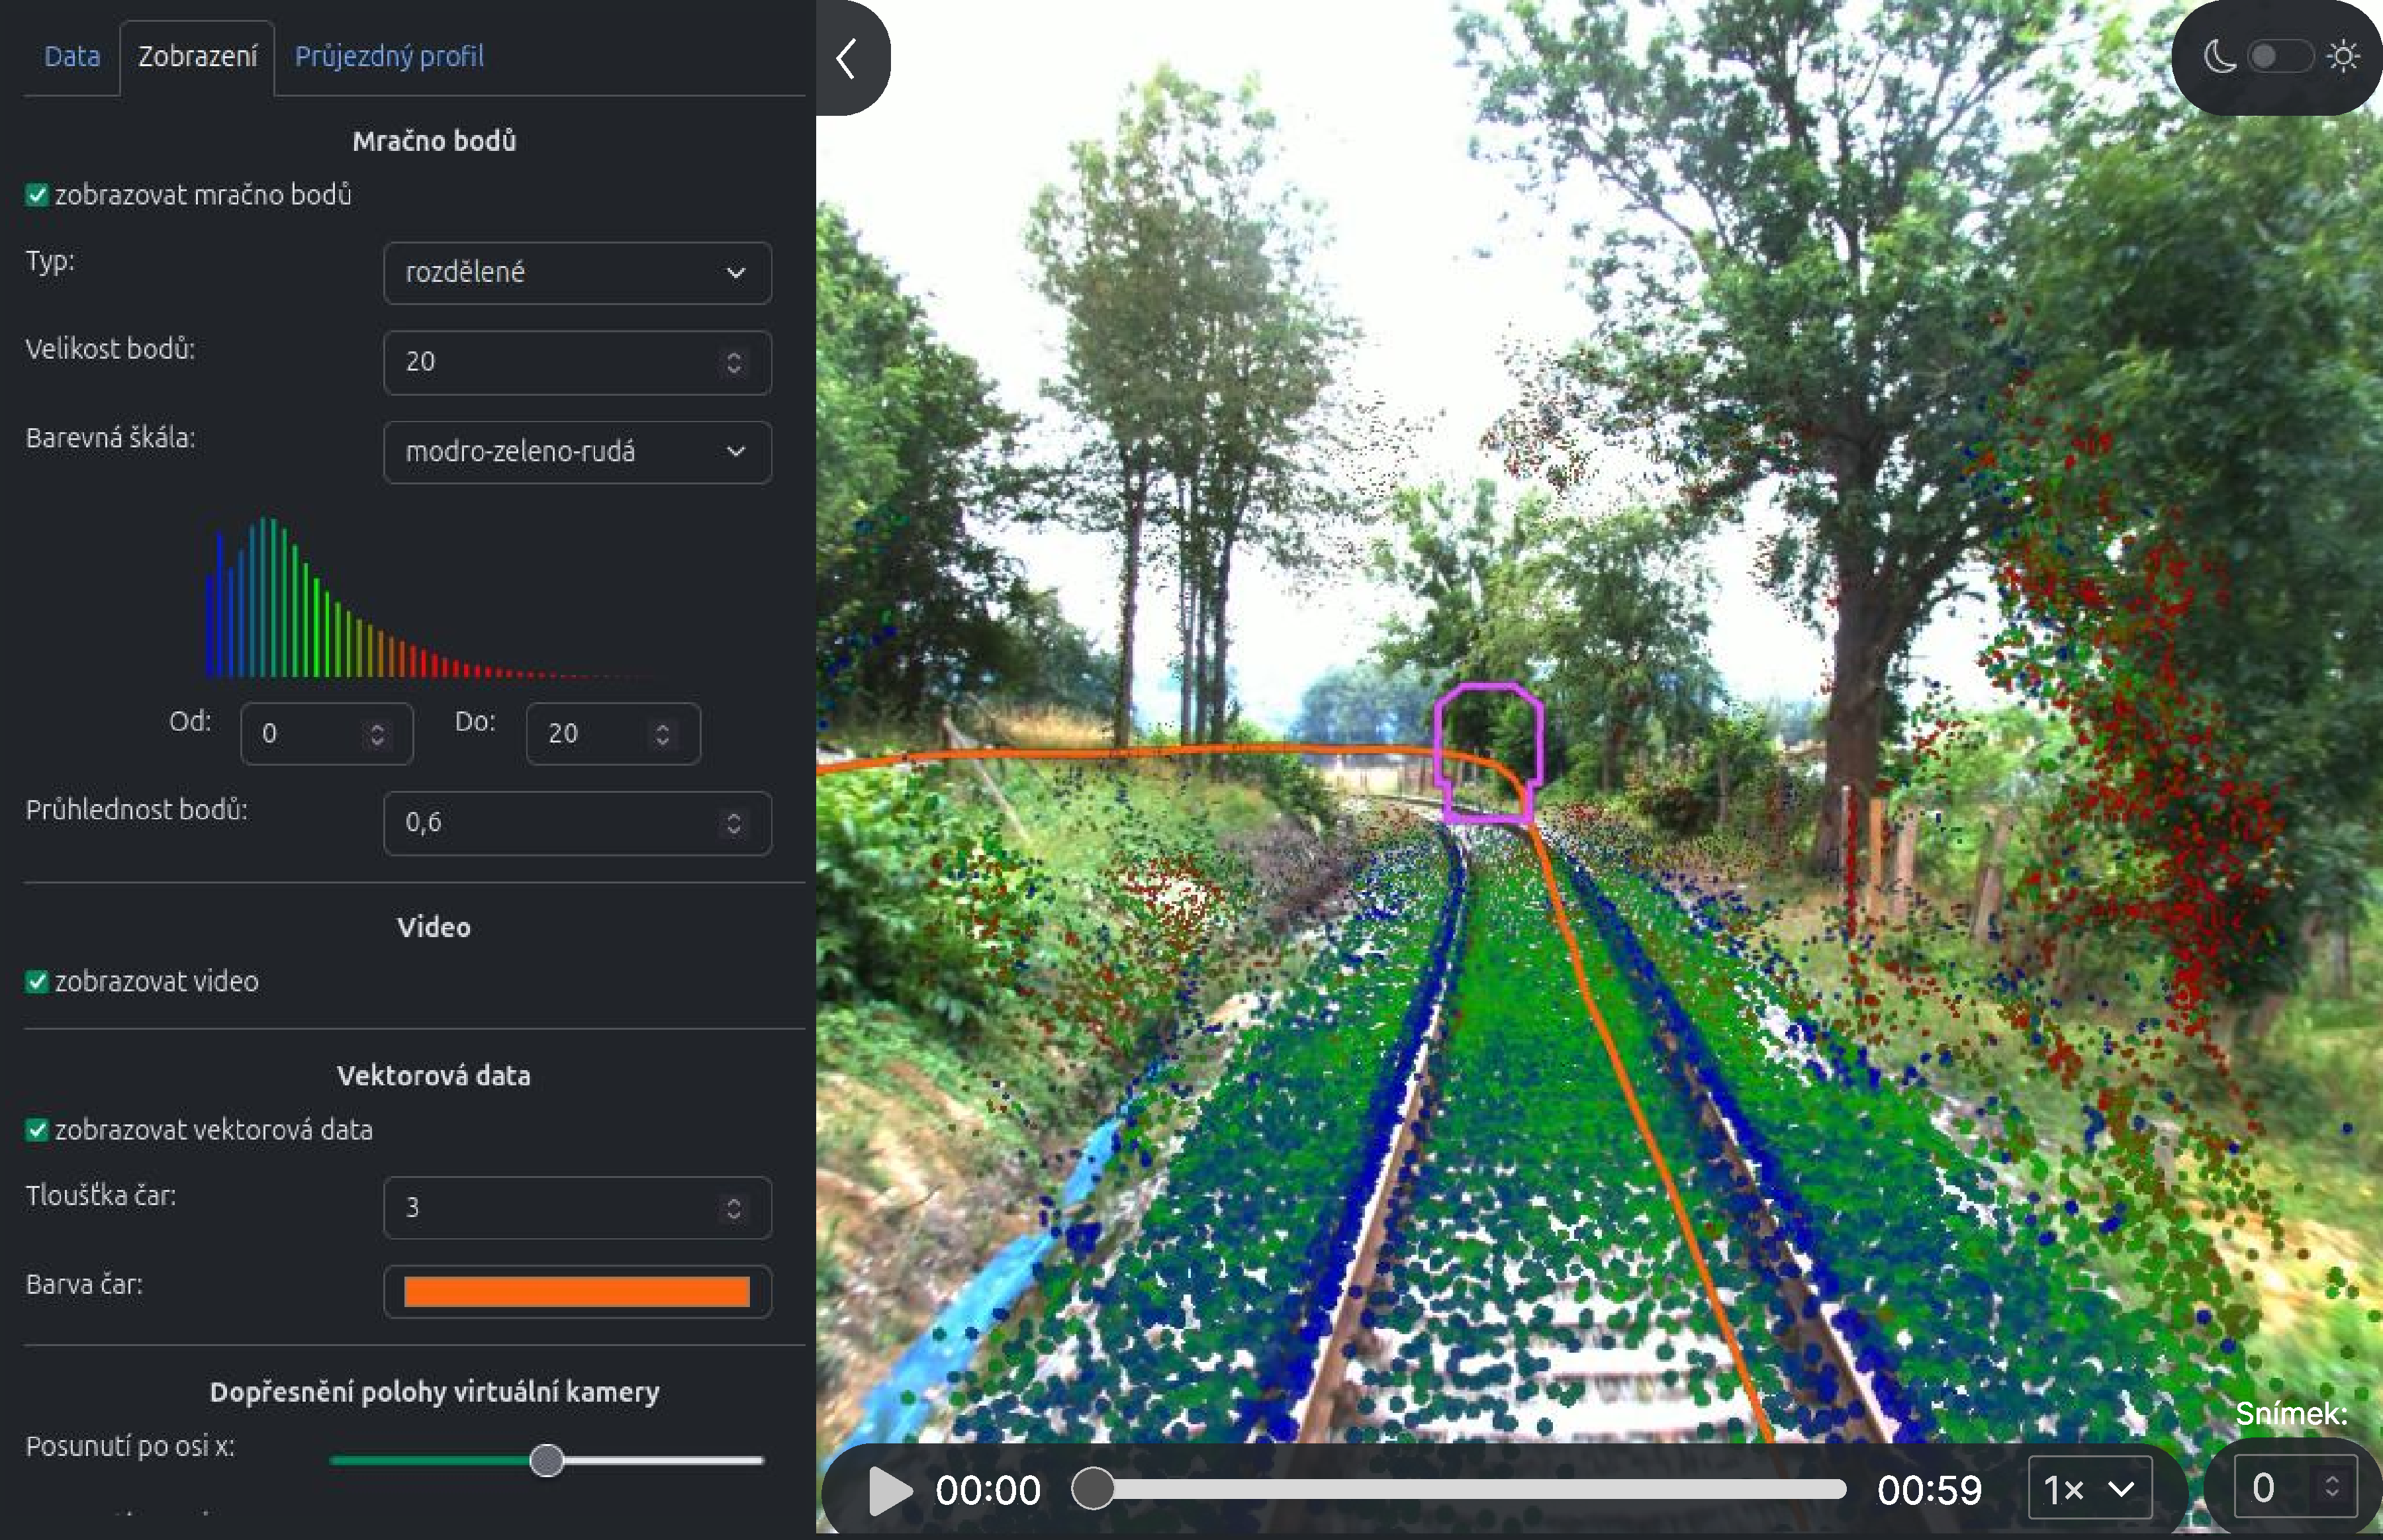
\includegraphics[width=0.9\linewidth]{text_prace/obrazky-figures/navrh2.pdf}
    \caption{Návrh používateľského rozhrania aplikácie vytvorený pomocou nástroja Figma.}
    \label{fig:navrh_gui}
\end{figure}

Hlavnou ideou návrhu je používanie čo najviac štandardných prvkov, aby sa v aplikácii používatelia ľahko zorientovali. Tomu napomáha aj použitie knižnice Bootstrap, ktorá je u webových aplikácií veľmi často používaná, a preto budú jej prvky pravdepodobne pre používateľov intuitívne.

Pre používateľskú prívetivosť by mala aplikácia spĺňať nasledujúce body:

\begin{enumerate}
    \item všeobecné vlastnosti:
    \begin{itemize}
        \item intuitívnosť,
        \item responzívny design,
        \item hladký beh animácií,
        \item možnosť exportu a importu nastavení zobrazenia,
        \item svetlý aj tmavý režim,
        \item kompatibilita s rôznymi prehliadačmi, prípadnú nekompatibilitu používateľovi ohlásiť,
    \end{itemize}
    \item v záložke \uv{Dáta}:
    \begin{itemize}
        \item prehľadné zobrazenie, aké dáta boli nahrané, možnosť ich nahradenia inými dátami,
        \item zobrazovanie indikátoru, že práve prebieha nahrávanie dát.
    \end{itemize}
\end{enumerate}

\section{Problém nahrávania dát do aplikácie}

Dáta, ktoré má vyvíjaná webová aplikácia zobrazovať, sú rozdelené do väčšieho množstva súborov rôznych typov. Nahrávať ich do aplikácie klasickým spôsobom po jednom či po nejakých skupinách by bolo síce možné, ale pre používateľov časovo náročné a veľmi nepraktické.

Keďže je aplikácia určená úzkej cieľovej skupine používateľov, môžeme si dovoliť predpokladať, že používateľ bude buď spúšťať server webovej aplikácie lokálne, alebo bude mať k~serveru aspoň prístup. Za tohto predpokladu má problém s~nahrávaním dát veľmi elegantné riešenie, a tým je \textbf{projektový súbor}, teda textový súbor, v~ktorom sú špecifikované cesty k~dátovým súborom uloženým na serveri. Používateľovi stačí nahrať tento súbor a aplikácia podľa neho automaticky nahrá všetky potrebné dátové súbory.

Presný formát projektového súboru bolo potrebné navrhnúť. Kompletný návrh je uvedený v~prílohe [DOPLNIŤ]. Bol zvolený formát TOML, ktorý je jednoduchý, praktický a dobre čitateľný \cite{toml}. U~dátových súborov, ktorých môže byť rôzny počet, napríklad súbory s~dátami z~lidaru, sa do projektového súboru uvedie, v~akom priečinku sa nachádzajú, ako sú pomenované a koľko ich je. Predpokladá sa, že sú tieto súbory jednotne pomenované a očíslované (napríklad \texttt{pcd\_0.pcd}, \texttt{pcd\_1.pcd}, \dots).

Keby však bol projektový súbor jediným možným spôsobom nahrávania dát do aplikácie, malo by to isté nevýhody -- napríklad pre vyskúšanie zmeny v~jednom dátovom súbore by bolo potrebné meniť projektový súbor a znova ho nahrávať.

Preto by mala výsledná aplikácia kombinovať oba prístupy, projektový súbor aj klasické nahrávanie dát. Pre jednoduchosť a prístupnosť by mala umožniť nahranie základných súborov klasickým spôsobom. Naopak pre pokročilejšie použitie by mala mať možnosť nahrania projektového súboru, podľa ktorého by mala nahrať všetky špecifikované dátové súbory. Potom by mal používateľ prehľadne vidieť všetky nahrané súbory a mať možnosť tieto súbory jednotlivo ľubovoľne nahradzovať inými súbormi.

\chapter{Implementácia navrhnutej aplikácie}

Navrhnutá webová aplikácia je implementovaná v jazyku Python s využitím frameworku Dash. Pre optimalizáciu obsahuje aplikácia aj skript napísaný v jazyku Javascript, ktorý používa pre vykresľovanie mračna bodov a vektorových dát framework deck.gl a na rozdiel od zvyšku kódu aplikácie sa vykonáva priamo na klientovi. Táto štruktúra je schematicky znázornená na obrázku \ref{fig:schema_implementacie}.

Zdrojový kód je rozdelený do nasledujúcich súborov:
\begin{itemize}
    \item \texttt{app.py} -- Hlavný súbor, inicializuje a spustí aplikáciu. Definuje základné rozloženie aplikácie -- vizualizácia na celú výšku okna, spodný panel a bočný panel so záložkami.
    \item \texttt{params.py} -- Počiatočné parametre.
    \item \texttt{loading\_functions.py} -- Pomocné funkcie pre načítanie dát zo súborov.
    \item \texttt{general\_functions.py} -- Pomocné funkcie pre výpočet projekčnej matice, transformačných matíc a operácií s rotáciami.
    \item Súbory s komponentmi a callbackmi rozdelené podľa štruktúry používateľského rozhrania:
    \begin{itemize}
        \item \texttt{animation\_control\_components.py}, \texttt{animation\_control\_callbacks.py} \\ -- komponenty v spodnom paneli,
        \item \texttt{data\_tab\_components.py}, \texttt{data\_tab\_callbacks.py}, \\\texttt{visualization\_tab\_components.py}, \texttt{visualization\_tab\_callbacks.py}, \\ \texttt{profile\_tab\_components.py}, \texttt{profile\_tab\_callbacks.py} \\ -- komponenty v záložkách v bočnom paneli.
    \end{itemize}
    \item \texttt{visualization.js} -- Vizualizácia mračna bodov a vektorových dát pomocou frameworku deck.gl, riadenie animácie phybu vlaku.
\end{itemize}

\begin{figure}[h]
    \centering
    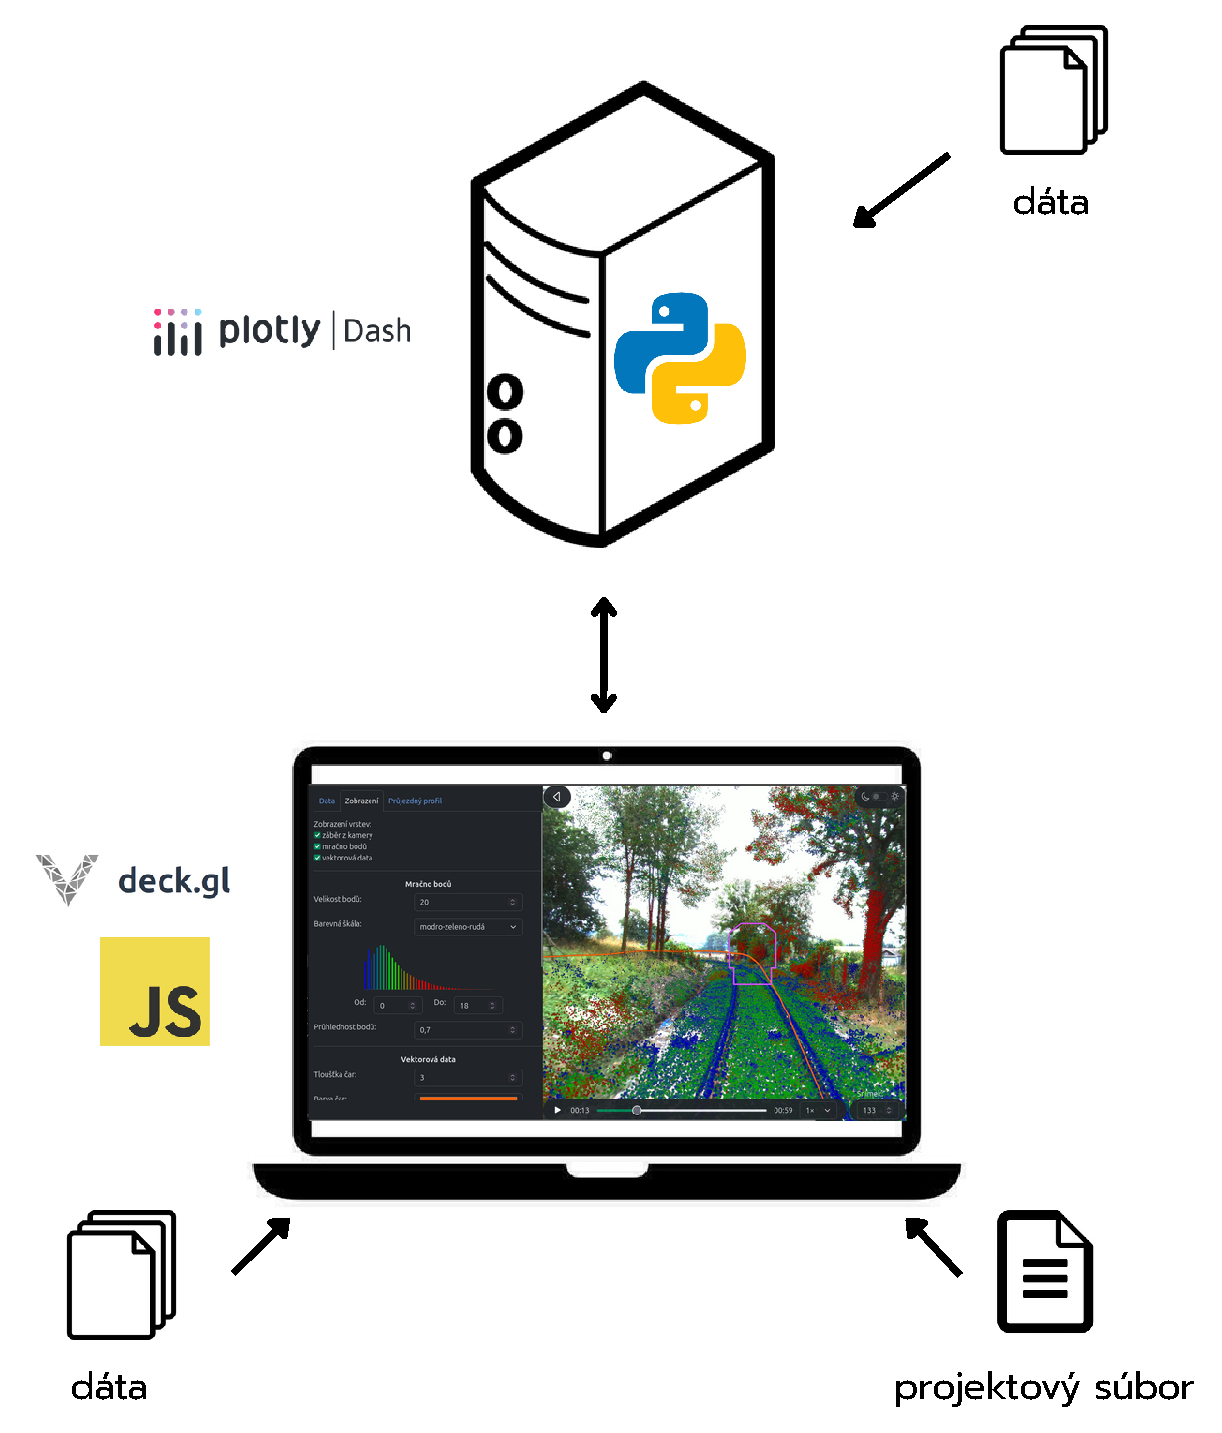
\includegraphics[width=0.7\linewidth]{text_prace/obrazky-figures/schema_implementacie.pdf}
    \caption{Schéma finálnej implementácie.}
    \label{fig:schema_implementacie}
\end{figure}

\section{Prvá etapa implementácie}

Prvým krokom implementácie bolo napísanie skriptu v~jazyku Python, ktorý vykresľoval mračno bodov bez použitia špeciálnych knižníc či frameworkov. K~dispozícii pritom bola jedna sada ukážkových dát, ktorá sa skladala z~mračna bodov, kalibračnej matice a postupnosti translácií a rotácií, ktoré predstavovali pohyb vlaku po trati. Mračno bodov obsahovalo 201~880 bodov s~intenzitou od 0 do 42 a bolo definovaných 500 polôh vlaku. K~tomu boli dodané obrázky, ktoré ukazovali, ako by mal vyzerať výsledok zobrazenia (obrázok \ref{fig:referencny-obrazok}).

\begin{figure}[h]
    \centering
    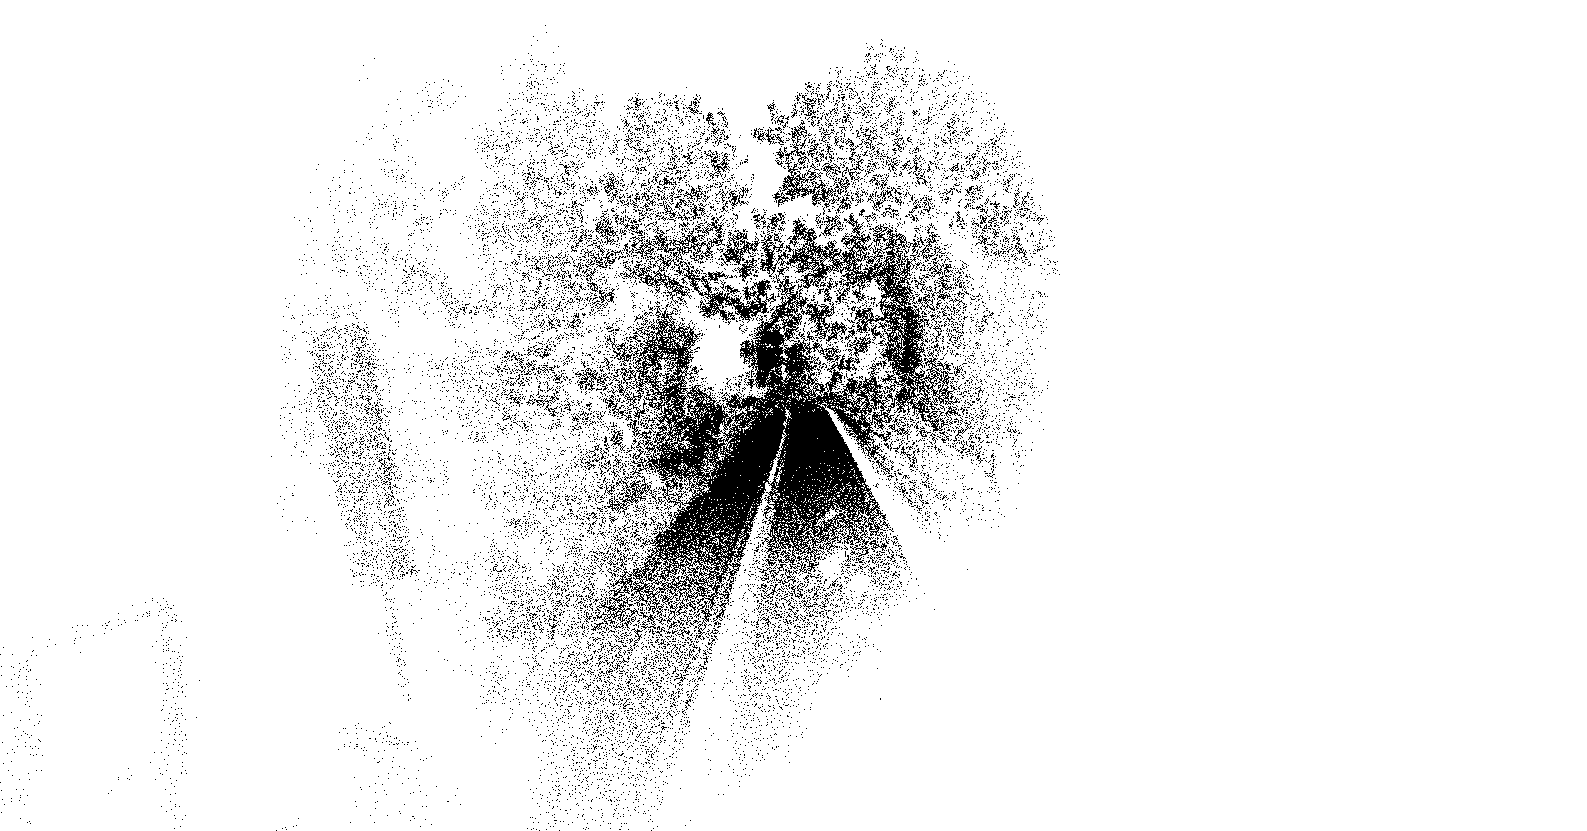
\includegraphics[width=0.95\linewidth]{obrazky-figures/referencny_obrazok.png}
    \caption{Referenčný obrázok, ktorý bol dodaný na začiatku práce spolu s~mračnom bodov a údajmi o~pohybe kamery v~ňom. Obrázok je tu pre lepšiu viditeľnosť s~invertovanými farbami a zväčšeným kontrastom.}
    \label{fig:referencny-obrazok}
\end{figure}

Cieľom tejto prvotnej fázy bolo najmä oboznámenie sa s~dátami a základnými princípmi vykresľovania bodov. Výsledky, ktoré sa nakoniec podarilo dosiahnuť, boli podobné referenčným obrázkom, aj keď nie úplne identické. Ukázalo sa, že údaje o~pohybe kamery majú iný súradnicový systém ako mračno bodov (líšilo sa poradie ôs) a že je potrebné pridať isté posunutie a rotáciu, aby sa výsledky podobali referenčným obrázkom (posunutie kamery do stredu vlaku, podľa dodaných dát bola naľavo od stredu).

Ďalej už nasledovala práca s~existujúcimi knižnicami a frameworkami v~jazyku Python. Prvotným plánom bolo použiť knižnicu Pydeck (pre vizualizáciu dát) s~frameworkom Streamlit (pre tvorbu GUI). Pydeck bol zvolený preto, že je nadstavbou nad javascriptovým frameworkom deck.gl, ktorý pri vykresľovaní dát využíva hardwarovú akceleráciu (GPU) a má dobrú výkonnosť. Ukázalo sa však, že Streamlit nepodporuje Pydeck v~plnej miere, a teda sa nedá využiť. Preto bol namiesto Streamlitu použitý framework Dash, ktorý už mal podporu pre Pydeck dostatočnú.

Pomocou tohto frameworku bola vytvorená jednoduchá webová aplikácia zobrazujúca ukážkové dáta a umožňujúca základné nastavenia vzhľadu. Do tejto aplikácie bolo zahrnuté aj zobrazovanie kamerového záznamu, pre tento účel bolo provizórne použité video z~prejazdu tej istej trate natočené v~roku 2012. Pri tom sa zistilo, že vykresľovanie dát pomocou kombinácie knižníc Pydeck a Dash Deck tak, ako je to vo vzorových príkladoch v~dokumentácii knižnice Dash Deck, je značne neefektívne. Jedno vykreslenie mračna bodov zaberalo zhruba 3 sekundy, čo bolo spôsobené transformáciami medzi rôznymi formátmi, ako to bolo popísané v~sekcii \ref{sec:deck_gl}.

Tento čas sa podarilo významne zredukovať použitím knižnice Dash Deck bez knižnice Pydeck. Výsledok však stále nebol dosť dobrý na to, aby mohla hladko bežať animácia pohybu vlaku, a ani napriek rôznym pokusom sa ho už nepodarilo v~rámci tejto kombinácie technológií vo významnejšej miere vylepšiť. Čas vykreslenia mračna bodov bol pritom úmerný počtu bodov a príčina neefektivity bola v~spôsobe implementácie knižnice Dash Deck. Bolo navyše potrebné rátať s~tým, že aplikácia bude zaťažená aj zobrazovaním videa. Preto bolo rozhodnuté optimalizovať vykresľovanie dát vynechaním knižnice Dash Deck a použitím frameworku deck.gl priamo z~jazyka Javascript.

\section{Optimalizácia vykresľovania mračna bodov}

Počas vývoja aplikácia prešla niekoľkými zmenami spôsobu vykresľovania mračna bodov a vektorových dát z dôvodu optimalizácie výkonu, ktoré sú popísané v nasledujúcich podsekciách.

Všetky v nich uvedené merania prebiehali na notebooku s~operačným systémom Ubuntu 24.04.1, procesorom Intel Core i5-9300H~×~8, grafickou kartou Intel UHD Graphics 630 (CFL GT2) a veľkosťou operačnej pamäte 16~GiB.

Profiling prebiehal v~prehliadači Google Chrome 133.0.6943.126 s~rozlíšením obrazovky 1480~×~832. Bol použitý profiler vstavaný v~tomto prehliadači.

\subsubsection{Optimalizácia priamym použitím frameworku deck.gl}

Aby bolo možné vynechať Dash Deck a použiť deck.gl priamo, bolo nutné nájsť spôsob, ako do aplikácie napísanej pomocou pythonového frameworku Dash zahrnúť kód v jazyku JavaScript, a zabezpečiť komunikáciu medzi týmto kódom a zvyškom aplikácie.

Dash interne používa na vytváranie používateľského rozhrania JavaScript, konkrétne framework React \cite{dash_documentation}. Jeho tvorcovia rátali s~tým, že vývojári, ktorí ho budú používať, budú niekedy chcieť priamo použiť javascriptový kód. Preto to tento framework umožňuje viacerými spôsobmi:

\begin{itemize}
    \item Klientske callbacky. Podobajú sa tým štandardným, ale na rozdiel od nich bežia iba na klientovi a píšu sa v~jazyku JavaScript. Štandardné callbacky bežia na serveri a píšu sa v~Pythone.
    \item Skripty v~jazyku JavaScript, ktoré je možné pripojiť k~generovanej HTML stránke. Spustia sa automaticky pri otvorení stránky v~prehliadači.
    \item Vytváranie vlastných komponentov používateľského rozhrania pomocou frameworku React.
\end{itemize}

V~tejto práci bola pre jednoduchosť využitá prvá a druhá možnosť. Bol napísaný skript \texttt{visualisation.js}, v~ktorom sú definované funkcie pre zobrazenie a zmeny zobrazenia dát pomocou deck.gl. Odkazy na tieto funkcie sú potom priradené do objektu \texttt{window}, aby bolo možné volať ich z~klientskych callbackov. Tento objekt teda tvorí rozhranie skriptu \texttt{visualisation.js}, ktoré je využívané zvyškom kódu aplikácie.

Pre správne pripojenie zdrojových kódov frameworku deck.gl k~javascriptovému kódu tak, aby mohol fungovať v~rámci aplikácie napísanej vo frameworku Dash, bolo nutné použiť bundler. V~rámci tejto práce bol použitý bundler Webpack. Výstupnému skriptu bolo potrebné nastaviť príponu \texttt{.mjs}, aby ho Dash spustil ako modul. Mimo modulu totiž nie je v jazyku JavaScript možné použiť deklaráciu \texttt{import}, ktorá je nutná pre pripojenie zdrojových kódov frameworku deck.gl.

\begin{table}[h]
    \centering
    \begin{tabular}{>{\centering\arraybackslash}m{10em}|>{\centering\arraybackslash}m{13em}|>{\centering\arraybackslash}m{12em}}
        {\RaggedRight Nastavenie parametra \texttt{interval} [ms]} &  {\RaggedRight Čas, za ktorý prebehla celá animácia (100 snímok) [s]} & {\RaggedRight Priemerný čas vykreslenia jednej snímky [ms]} \\ \hline
        1000 & 101 & 1010 \\
        800 & 80 & 800 \\
        750 & 76 & 760 \\
        700 & 72 & 720 \\
        650 & 71 & 710 \\
        600 & 70 & 700 \\
    \end{tabular}
    \caption{Výkonnosť vykresľovania mračna bodov obsahujúceho 201~880 bodov \emph{pred prvou optimalizáciou}, teda iba pomocou kódu v~jazyku Python. Použité technológie: Python, Dash, Dash Deck. Z~nameraných údajov vyplýva, že minimálny čas potrebný vykreslenie jednej snímky je asi 750~ms, čo znamená, že rýchlosť nedosahuje ani 2 snímky za sekundu.}
    \label{tab:js_optimalizacia_pred}
\end{table}

\begin{table}[h]
    \centering
    \begin{tabular}{>{\centering\arraybackslash}m{10em}|>{\centering\arraybackslash}m{13em}|>{\centering\arraybackslash}m{12em}}
         Nastavenie parametra \texttt{interval} [ms] &  Čas, za ktorý prebehla celá animácia (500 snímok) [s] & Priemerný čas vykreslenia jednej snímky [ms] \\ \hline
        250 & 126 & 252 \\
        200 & 101 & 202 \\
        150 & 76 & 152 \\
        125 & 68 & 136 \\
        100 & 63 & 126 \\
         75 & 62 & 124 \\
    \end{tabular}
    \caption{Výkonnosť vykresľovania mračna bodov obsahujúceho 201~880 bodov \emph{po prvej optimalizácii}, teda s~vykresľovaním dát v~jazyku Javascript. Použité technológie: Python, Dash, Javascript, deck.gl. Z~nameraných údajov vyplýva, že minimálny čas potrebný vykreslenie jednej snímky je asi 150~ms, čo zodpovedá rýchlosti asi 6 snímok za sekundu.}
    \label{tab:js_optimalizacia_po}
\end{table}

Meraná bola výkonnosť vykresľovania mračna bodov počas animácie pohybu vlaku. Animácia bola riadená pomocou komponentu \texttt{Interval} frameworku Dash, ktorého funkcionalita spočíva v tom, že periodicky spúšťa callback, pričom periódu určuje parameter \texttt{interval}.

Meranie výkonnosti vykresľovania mračna bodov pred a po optimalizácii je popísané v~tabuľkách \ref{tab:js_optimalizacia_pred} a \ref{tab:js_optimalizacia_po}.

Z dát v tabuľkách vyplýva, že optimalizácia výkon výrazne zlepšila. 

\subsubsection{Optimalizácia riadením animácie výhradne na strane klienta}

Optimalizácia popísaná v predchádzajúcej podsekcii síce priniesla z hľadiska výkonu zlepšenie, ale výsledok stále nebol dostačujúci. 

Riadenie animácie pomocou komponentu \texttt{Interval} frameworku Dash je totiž pomerne ťažkopádne, pretože funguje na základe komunikácie medzi klientom a serverom a tým animáciu spomaľuje. Preto bolo vhodné nahradiť ho riadením animácie v~jazyku JavaScript výhradne na strane klienta.

Podrobný popis tohto spôsobu riadenia animácie je uvedený v sekcii \ref{sec:implementacia_animacie}.

\begin{figure}[h!]
    \centering
    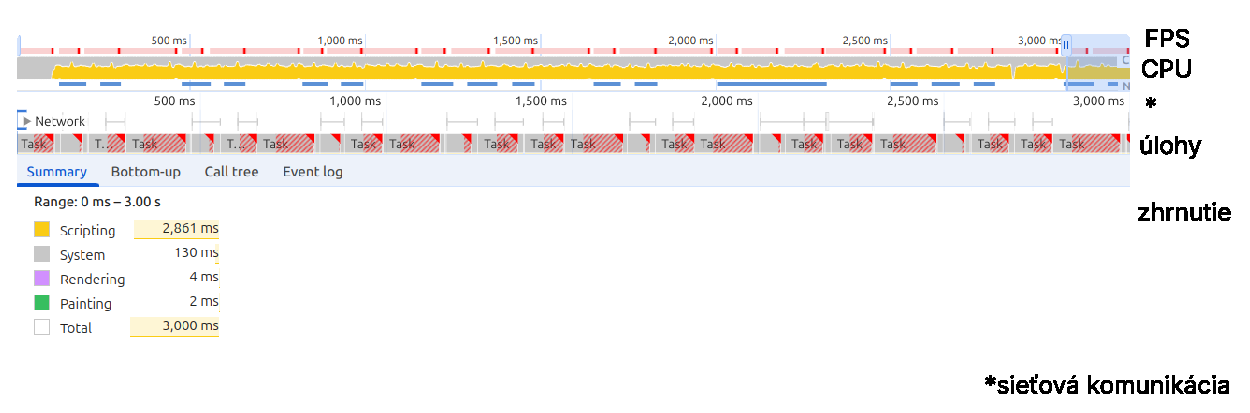
\includegraphics[width=1\linewidth]{text_prace/obrazky-figures/profiling_interval.pdf}
    \caption{Profiling animácie pohybu vlaku, ktorá je riadená pomocou komponentu \texttt{Interval}.}
    \label{fig:profiling_interval}
\end{figure}

\begin{figure}[h!]
    \centering
    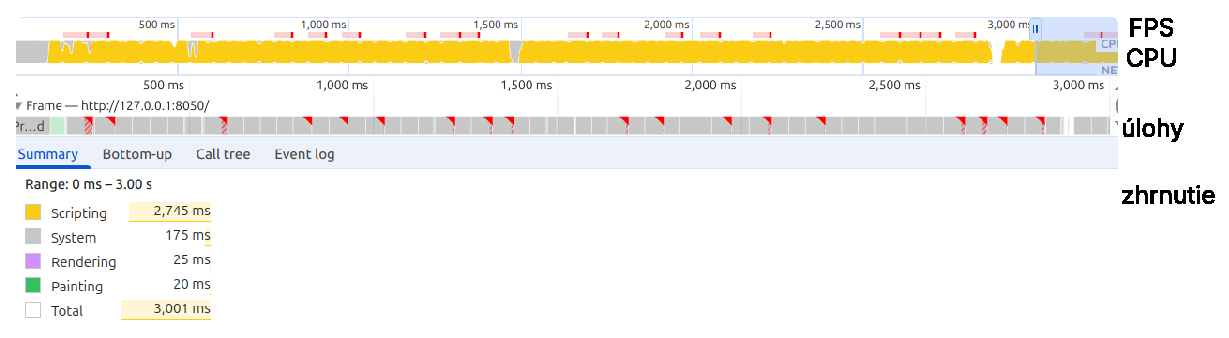
\includegraphics[width=1\linewidth]{text_prace/obrazky-figures/profiling1.pdf}
    \caption{Profiling animácie pohybu vlaku, ktorá je riadená iba pomocou kódu v jazyku JavaScript.}
    \label{fig:profiling1}
\end{figure}

Oba spôsoby boli porovnané pomocou profilingu. V~aplikácii sa prehrávala animácia pohybu kamery spojená s~videom. Vizualizované dáta tvorila jedna vrstva \texttt{PointCloudLayer}, ktorá obsahovala 201~880 bodov. Výsledky profilingu sú na obrázkoch \ref{fig:profiling_interval} a \ref{fig:profiling1}.

Z grafov je možné vyčítať, že hoci sa zvýšilo zaťaženie procesora, výrazne sa znížil čas potrebný na vykreslenie jednej snímky animácie, čo umožnilo vykreslenie väčšieho počtu snímok za sekundu (v grafoch sekcia \uv{úlohy}).

Animácia teda bežala hladšie, ale výkon aplikácie stále nebol vyhovujúci, pretože animácia výrazne zaťažovala procesor a hodnota snímkovej frekvencie stále miestami dosahovala príliš nízke hodnoty (v grafoch červené čiary v sekcii \uv{FPS}).

\subsubsection{Optimalizácia použitím iného spôsobu nastavenia polohy kamery}

V~sekcii \ref{sec:nastavenie_polohy_kamery} boli popísané dva rôzne spôsoby nastavenia polohy kamery vo frameworku deck.gl. V~implementácii aplikácie bol použitý najprv prvý spôsob, teda aplikovanie transformácií na dáta, pretože bol jednoduchší a priamo vyplynul z~prvej fázy implementácie (vykreslenie mračna bodov v~jazyku Python bez použitia frameworku). Ten bol následne zmenený na druhý spôsob, teda aplikovanie transformácií na kameru, pretože sa ukázalo, že tak dôjde k~významnej optimalizácii.

Nový spôsob nastavenia polohy kamery bol analyzovaný pomocou profilingu rovnakej animácie ako v prechádzajúcej podsekcii.

\begin{figure}[h!]
    \centering
    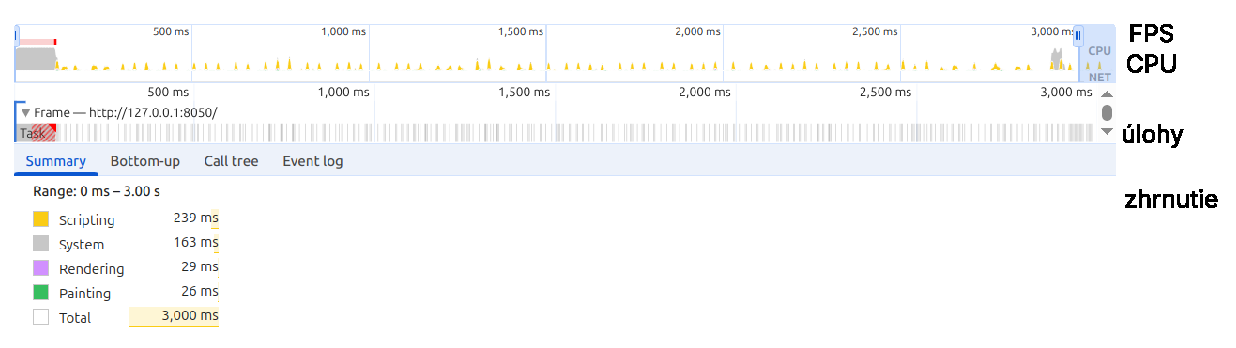
\includegraphics[width=1\linewidth]{text_prace/obrazky-figures/profiling2.pdf}
    \caption{Profiling animácie pohybu vlaku s novým spôsobom nastavenia polohy kamery.}
    \label{fig:profiling2}
\end{figure}

Z~nameraných údajov vyplýva, že táto optimalizácia veľmi výrazne znížila zaťaženie procesora. Zatiaľ čo pred optimalizáciou (obr. \ref{fig:profiling1}) sa počas trojsekudového intervalu vykonával javascriptový kód 2,745 sekúnd, po optimalizácii (obr. \ref{fig:profiling2}) to bolo iba 239 milisekúnd, čo predstavuje viac než desaťnásobné zníženie.

Dôležitou metrikou pri posudzovaní výkonnosti animácií je snímková frekvencia meraná v~FPS (\emph{frames per second}, počet vykreslených snímok za sekundu). V~ideálnom prípade by sa snímková frekvencia mala blížiť 60~FPS, pretože vtedy sa animácia ľudskému oku zdá hladká \cite{chrome_profiling}.

Podľa vstavaného ukazovateľa snímkovej frekvencie v~prehliadači Google Chrome dosahovala skúmaná animácia pred optimalizáciu zhruba 28 až 34~FPS, zatiaľ čo po nej 51 až 55~FPS. Aj v~tomto ohľade teda nastalo významné zlepšenie.

\section{Rozdelenie dát do vrstiev}

Pri vizualizácii dát pomocou frameworku deck.gl sú použité dva typy vrstiev:
\begin{itemize}
    \item \texttt{PointCloudLayer} pre mračno bodov,
    \item \texttt{PathLayer} pre vektorové dáta.
\end{itemize}
Rozdelenie vizualizácie na vrstvy je znázornené na obrázku \ref{fig:vrstvy}.

\begin{figure}[h]
    \centering
    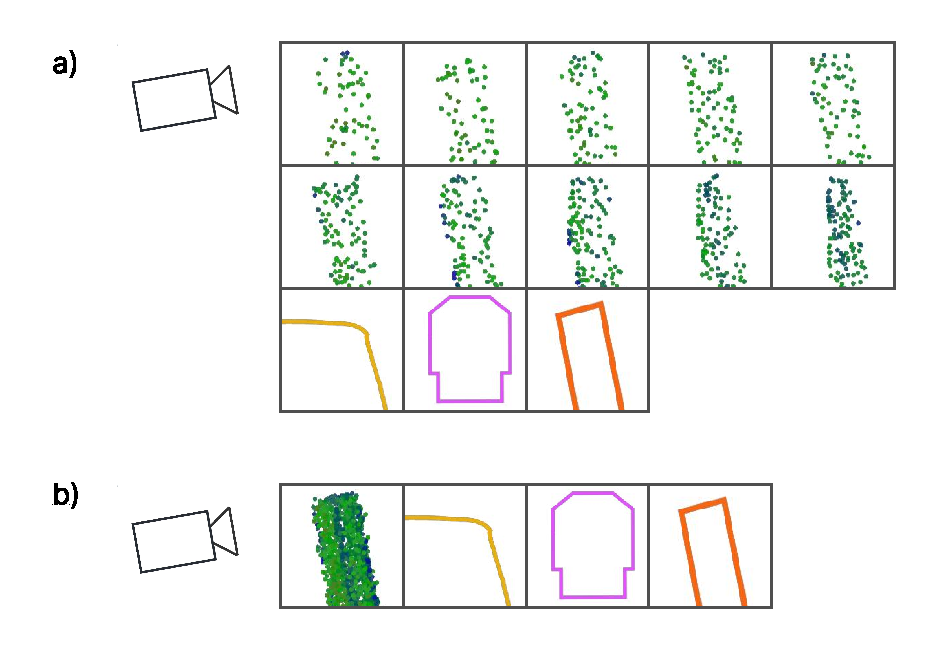
\includegraphics[width=0.8\linewidth]{text_prace/obrazky-figures/vrstvy.pdf}
    \caption{Schéma rozdelenia dát do vrstiev. Počet vrstiev s mračnom bodov závisí od typu zobrazovaného mračna bodov.}
    \label{fig:vrstvy}
\end{figure}

Na začiatku tvorby práce bola na zobrazenie vektorových dát použitá vrstva \texttt{LineLayer}. Ukázalo sa však, že vstva \texttt{LineLayer} je prispôsobená iba pre zobrazovanie čiar na mapách a pri použití nemapového pohľadu ako \texttt{FirstPersonView} nefunguje dobre -- niektoré čiary sa otáčajú kolmo ku kamere a tým pádom sa ich šírka zmenšuje, niekedy až tak, že úplne prestanú byť viditeľné. Toto správanie u vrstvy \texttt{LineLayer} nie je možné zmeniť. Naopak u vrstvy \texttt{PathLayer} je možné nastaviť vlastnosť \texttt{billboard}, ktorá znamená otočenie čiar smerom ku kamere, preto bola nakoniec táto vrstva použitá namiesto vrstvy \texttt{LineLayer}. \texttt{PathLayer} sa od \texttt{LineLayer} líši ešte tým, že čiary majú pevnú šírku v pixeloch a nezužujú sa podľa toho, ako ďaleko sú od kamery.

Vizualizácia obsahuje nasledujúce vrstvy:
\begin{itemize}
    \item Mračno bodov. Ak aplikácia zobrazuje \emph{rozdelené} mračno bodov, teda malé, postupne nasnímané časti s časovými razítkami, tak je vrstiev desať a zobrazujú desať z týchto častí -- jednu, ktorá zodpovedá danej pozícii, a deväť predchádzajúcich (obrázok \ref{fig:vrstvy}, časť a)). Ak aplikácia zobrazuje \emph{celistvé} mračno bodov, tak je celé v jednej vrstve (obrázok \ref{fig:vrstvy}, časť b)).
    \item Čiara spájajúca predikované polohy prejazdného profilu vlaku.
    \item Prejazdný profil vlaku v predikovanej polohe. Od ostatných vektorových dát sa líši tým, že sa jeho poloha mení pri zmene polohy kamery. To je v implementácii dosiahnuté pomocou špeciálnej prístupovej funkcie \texttt{profileGetPath} (prístupové funkcie boli popísané v sekcii \ref{sec:nastavenie_polohy_kamery}, podsekcia Aplikovanie transformácií na dáta). 
    \item Ďalšie vektorové dáta.
\end{itemize}

\subsubsection{Farebné škály}

Okrem polohy má každý bod v mračne bodov v dodanej sade dát určenú ešte jednu vlastnosť -- intenzitu v rozmedzí od 0 do 42, ktorú je vhodné farebne rozlíšiť.

Boli implementované dve farebné škály, klasická modro-zeleno-červená a žlto-fialová, pričom u oboch si môže používateľ zvoliť, od akej intenzity začína a pri akej končí. Ak je napríklad nastavená žlto-fialová farebná škála od 0 do 20, tak to znamená, že body s intenzitou 0 budú mať žltú farbu, body s intenzitou 20 a vyššou fialovú farbu a body s intenzitou od 1 do 19 kombinovanú farbu.

Pre prehľadnosť bol tiež implementovaný graf, ktorý používateľovi ukazuje relatívne počty bodov s jednotlivými intenzitami a aké majú nastavené farby. Ukážky možných nastavení sú na obrázku \ref{fig:farebna_skala}.

\begin{figure}[h]
    \centering
    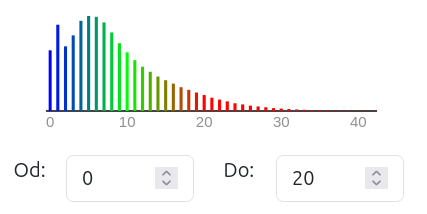
\includegraphics[width=0.35\linewidth]{text_prace/obrazky-figures/farebna_skala1.png}
    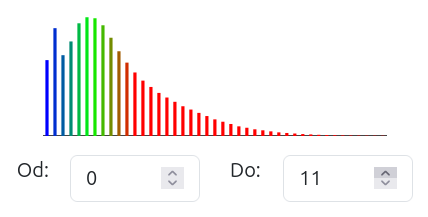
\includegraphics[width=0.35\linewidth]{text_prace/obrazky-figures/farebna_skala2.png}
    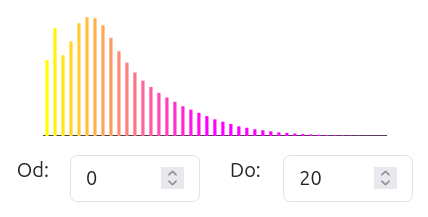
\includegraphics[width=0.35\linewidth]{text_prace/obrazky-figures/farebna_skala3.png}
    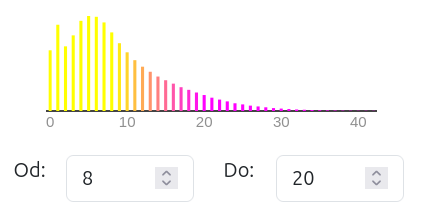
\includegraphics[width=0.35\linewidth]{text_prace/obrazky-figures/farebna_skala4.png}
    \caption{Nastaviteľná farebná škála pre mračno bodov. Vodorovná os predstavuje intenzitu, vertikálna os predstavuje počet bodov.}
    \label{fig:farebna_skala}
\end{figure}

\section{Implementácia animácie pohybu vlaku}
\label{sec:implementacia_animacie}

[obrázok prepisovania vrstiev]

\section{Implementácia skreslenia}


\chapter{Testovanie}

\section{Zobrazenie dodaných dát}

% Užitočná by bola aj možnosť doladiť parametre zobrazovania mračna bodov a vektorových dát (posun aj otočenie kamery doprava/doľava, nahor/nadol, posun dopredu/dozadu), aby bolo možné toto zobrazenie prispôsobiť záznamu z~kamery. Kamera totiž môže byť na vlaku rôzne umiestnená a údaje z~nej môžu byť oproti údajom z~mračna bodov posunuté.

\section{Výkonnosť}

\section{Vyhodnotenie používateľskej prívetivosti}

\chapter{Záver}


%===============================================================================

% Pro kompilaci po částech (viz projekt.tex) nutno odkomentovat
%\end{document}
